\documentclass[11pt]{article}
\usepackage[letterpaper, top=0.7in, bottom=0.75in, left=0.7in, right=0.7in,
  headheight=15pt, headsep=12pt, footskip=26pt]{geometry}
\usepackage[T1]{fontenc}
\usepackage{helvet}
\renewcommand{\familydefault}{\sfdefault}
\usepackage{tikz}
\usetikzlibrary{arrows.meta}
\usepackage{fancyhdr}
\pagestyle{fancy}
\fancyhf{}
\lhead{Week 63 / Cards away from home / Grades 2--3}
\lfoot{Bellingham Math Circle / Week 63 / W63-RV-M-v1}
\rfoot{\thepage}
\renewcommand{\headrulewidth}{0.4pt}
\setlength{\parindent}{0pt}
\setlength{\parskip}{0pt}
\newcommand{\prob}[1]{\textbf{Problem #1:}}
\begin{document}
The homes stay in place. A card is at home when it sits in the home with its own letter. A swap trades the places of any two cards, near or far. Write each swap as the letters of the two cards it trades.

\par\vspace{3mm}\noindent\hspace*{30mm}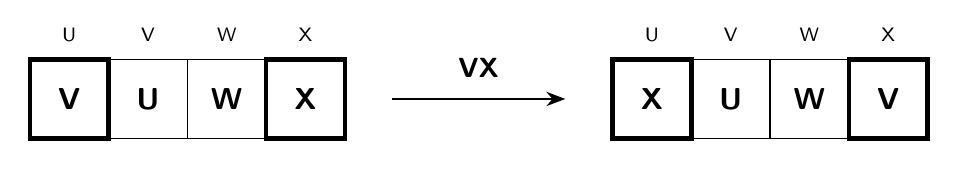
\begin{tikzpicture}[x=1mm, y=1mm]
\draw[line width=1.6pt] (0,0) rectangle (10,10);
\node[inner sep=0, font=\fontsize{7}{8.4}\selectfont] at (5,13.2) {U};
\node[inner sep=0, font=\fontsize{11}{13.2}\selectfont\bfseries] at (5,5) {V};
\draw[line width=0.6pt] (10,0) rectangle (20,10);
\node[inner sep=0, font=\fontsize{7}{8.4}\selectfont] at (15,13.2) {V};
\node[inner sep=0, font=\fontsize{11}{13.2}\selectfont\bfseries] at (15,5) {U};
\draw[line width=0.6pt] (20,0) rectangle (30,10);
\node[inner sep=0, font=\fontsize{7}{8.4}\selectfont] at (25,13.2) {W};
\node[inner sep=0, font=\fontsize{11}{13.2}\selectfont\bfseries] at (25,5) {W};
\draw[line width=1.6pt] (30,0) rectangle (40,10);
\node[inner sep=0, font=\fontsize{7}{8.4}\selectfont] at (35,13.2) {X};
\node[inner sep=0, font=\fontsize{11}{13.2}\selectfont\bfseries] at (35,5) {X};
\draw[-{Stealth[length=2.4mm]}, line width=0.9pt] (46,5) -- (68,5);
\node[font=\fontsize{10}{12.0}\selectfont\bfseries] at (57,9) {VX};
\draw[line width=1.6pt] (74,0) rectangle (84,10);
\node[inner sep=0, font=\fontsize{7}{8.4}\selectfont] at (79,13.2) {U};
\node[inner sep=0, font=\fontsize{11}{13.2}\selectfont\bfseries] at (79,5) {X};
\draw[line width=0.6pt] (84,0) rectangle (94,10);
\node[inner sep=0, font=\fontsize{7}{8.4}\selectfont] at (89,13.2) {V};
\node[inner sep=0, font=\fontsize{11}{13.2}\selectfont\bfseries] at (89,5) {U};
\draw[line width=0.6pt] (94,0) rectangle (104,10);
\node[inner sep=0, font=\fontsize{7}{8.4}\selectfont] at (99,13.2) {W};
\node[inner sep=0, font=\fontsize{11}{13.2}\selectfont\bfseries] at (99,5) {W};
\draw[line width=1.6pt] (104,0) rectangle (114,10);
\node[inner sep=0, font=\fontsize{7}{8.4}\selectfont] at (109,13.2) {X};
\node[inner sep=0, font=\fontsize{11}{13.2}\selectfont\bfseries] at (109,5) {V};
\end{tikzpicture}\par

\vspace{8mm}
\prob{1} Start with A, B, C and D at home. Swap cards until no card is at home, using as few swaps as you can. Which rows can you end with in that many swaps? Then find the fewest swaps for all five cards.

\par\vspace{3mm}\noindent\hspace*{2mm}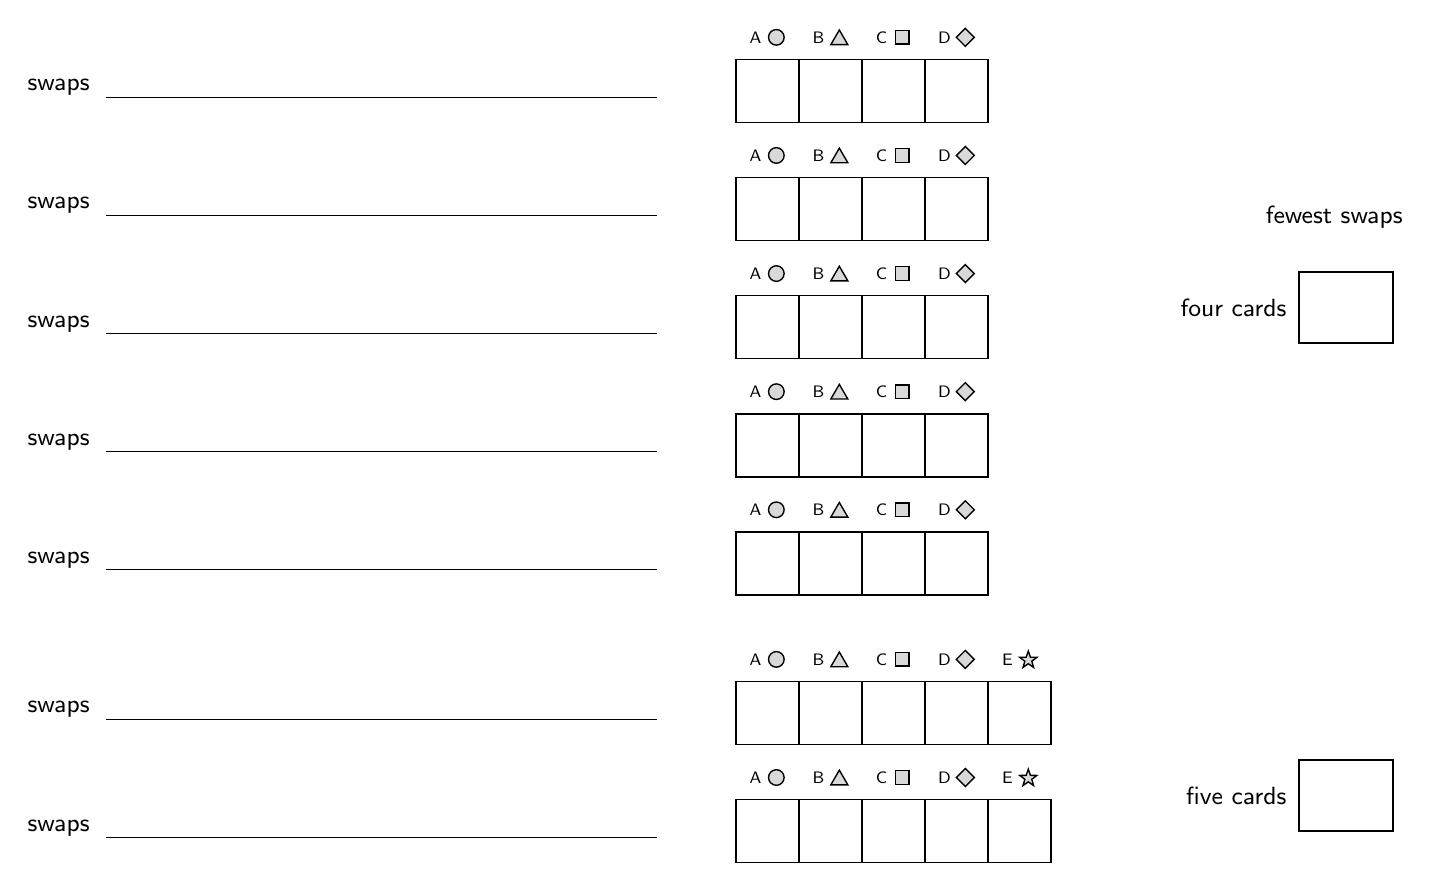
\begin{tikzpicture}[x=1mm, y=1mm]
\node[anchor=base west, inner sep=0, font=\fontsize{9}{10.8}\selectfont] at (0,2) {swaps};
\draw[line width=0.4pt] (10.05,1.2) -- (80.05,1.2);
\draw[line width=0.6pt] (90,-2) rectangle (98,6);
\node[inner sep=0, font=\fontsize{6}{7.2}\selectfont] at (92.5,8.8) {A};
\path[fill=gray!30, draw=black, line width=0.5pt] (95.15,8.8) circle (0.99);
\draw[line width=0.6pt] (98,-2) rectangle (106,6);
\node[inner sep=0, font=\fontsize{6}{7.2}\selectfont] at (100.5,8.8) {B};
\path[fill=gray!30, draw=black, line width=0.5pt] (103.15,9.73) -- (102.07,7.87) -- (104.23,7.87) -- cycle;
\draw[line width=0.6pt] (106,-2) rectangle (114,6);
\node[inner sep=0, font=\fontsize{6}{7.2}\selectfont] at (108.5,8.8) {C};
\path[fill=gray!30, draw=black, line width=0.5pt] (110.29,7.94) rectangle (112.01,9.66);
\draw[line width=0.6pt] (114,-2) rectangle (122,6);
\node[inner sep=0, font=\fontsize{6}{7.2}\selectfont] at (116.5,8.8) {D};
\path[fill=gray!30, draw=black, line width=0.5pt] (119.15,9.94) -- (120.29,8.8) -- (119.15,7.66) -- (118.01,8.8) -- cycle;
\node[anchor=base west, inner sep=0, font=\fontsize{9}{10.8}\selectfont] at (0,-13) {swaps};
\draw[line width=0.4pt] (10.05,-13.8) -- (80.05,-13.8);
\draw[line width=0.6pt] (90,-17) rectangle (98,-9);
\node[inner sep=0, font=\fontsize{6}{7.2}\selectfont] at (92.5,-6.2) {A};
\path[fill=gray!30, draw=black, line width=0.5pt] (95.15,-6.2) circle (0.99);
\draw[line width=0.6pt] (98,-17) rectangle (106,-9);
\node[inner sep=0, font=\fontsize{6}{7.2}\selectfont] at (100.5,-6.2) {B};
\path[fill=gray!30, draw=black, line width=0.5pt] (103.15,-5.27) -- (102.07,-7.13) -- (104.23,-7.13) -- cycle;
\draw[line width=0.6pt] (106,-17) rectangle (114,-9);
\node[inner sep=0, font=\fontsize{6}{7.2}\selectfont] at (108.5,-6.2) {C};
\path[fill=gray!30, draw=black, line width=0.5pt] (110.29,-7.06) rectangle (112.01,-5.34);
\draw[line width=0.6pt] (114,-17) rectangle (122,-9);
\node[inner sep=0, font=\fontsize{6}{7.2}\selectfont] at (116.5,-6.2) {D};
\path[fill=gray!30, draw=black, line width=0.5pt] (119.15,-5.06) -- (120.29,-6.2) -- (119.15,-7.34) -- (118.01,-6.2) -- cycle;
\node[anchor=base west, inner sep=0, font=\fontsize{9}{10.8}\selectfont] at (0,-28) {swaps};
\draw[line width=0.4pt] (10.05,-28.8) -- (80.05,-28.8);
\draw[line width=0.6pt] (90,-32) rectangle (98,-24);
\node[inner sep=0, font=\fontsize{6}{7.2}\selectfont] at (92.5,-21.2) {A};
\path[fill=gray!30, draw=black, line width=0.5pt] (95.15,-21.2) circle (0.99);
\draw[line width=0.6pt] (98,-32) rectangle (106,-24);
\node[inner sep=0, font=\fontsize{6}{7.2}\selectfont] at (100.5,-21.2) {B};
\path[fill=gray!30, draw=black, line width=0.5pt] (103.15,-20.27) -- (102.07,-22.13) -- (104.23,-22.13) -- cycle;
\draw[line width=0.6pt] (106,-32) rectangle (114,-24);
\node[inner sep=0, font=\fontsize{6}{7.2}\selectfont] at (108.5,-21.2) {C};
\path[fill=gray!30, draw=black, line width=0.5pt] (110.29,-22.06) rectangle (112.01,-20.34);
\draw[line width=0.6pt] (114,-32) rectangle (122,-24);
\node[inner sep=0, font=\fontsize{6}{7.2}\selectfont] at (116.5,-21.2) {D};
\path[fill=gray!30, draw=black, line width=0.5pt] (119.15,-20.06) -- (120.29,-21.2) -- (119.15,-22.34) -- (118.01,-21.2) -- cycle;
\node[anchor=base west, inner sep=0, font=\fontsize{9}{10.8}\selectfont] at (0,-43) {swaps};
\draw[line width=0.4pt] (10.05,-43.8) -- (80.05,-43.8);
\draw[line width=0.6pt] (90,-47) rectangle (98,-39);
\node[inner sep=0, font=\fontsize{6}{7.2}\selectfont] at (92.5,-36.2) {A};
\path[fill=gray!30, draw=black, line width=0.5pt] (95.15,-36.2) circle (0.99);
\draw[line width=0.6pt] (98,-47) rectangle (106,-39);
\node[inner sep=0, font=\fontsize{6}{7.2}\selectfont] at (100.5,-36.2) {B};
\path[fill=gray!30, draw=black, line width=0.5pt] (103.15,-35.27) -- (102.07,-37.13) -- (104.23,-37.13) -- cycle;
\draw[line width=0.6pt] (106,-47) rectangle (114,-39);
\node[inner sep=0, font=\fontsize{6}{7.2}\selectfont] at (108.5,-36.2) {C};
\path[fill=gray!30, draw=black, line width=0.5pt] (110.29,-37.06) rectangle (112.01,-35.34);
\draw[line width=0.6pt] (114,-47) rectangle (122,-39);
\node[inner sep=0, font=\fontsize{6}{7.2}\selectfont] at (116.5,-36.2) {D};
\path[fill=gray!30, draw=black, line width=0.5pt] (119.15,-35.06) -- (120.29,-36.2) -- (119.15,-37.34) -- (118.01,-36.2) -- cycle;
\node[anchor=base west, inner sep=0, font=\fontsize{9}{10.8}\selectfont] at (0,-58) {swaps};
\draw[line width=0.4pt] (10.05,-58.8) -- (80.05,-58.8);
\draw[line width=0.6pt] (90,-62) rectangle (98,-54);
\node[inner sep=0, font=\fontsize{6}{7.2}\selectfont] at (92.5,-51.2) {A};
\path[fill=gray!30, draw=black, line width=0.5pt] (95.15,-51.2) circle (0.99);
\draw[line width=0.6pt] (98,-62) rectangle (106,-54);
\node[inner sep=0, font=\fontsize{6}{7.2}\selectfont] at (100.5,-51.2) {B};
\path[fill=gray!30, draw=black, line width=0.5pt] (103.15,-50.27) -- (102.07,-52.13) -- (104.23,-52.13) -- cycle;
\draw[line width=0.6pt] (106,-62) rectangle (114,-54);
\node[inner sep=0, font=\fontsize{6}{7.2}\selectfont] at (108.5,-51.2) {C};
\path[fill=gray!30, draw=black, line width=0.5pt] (110.29,-52.06) rectangle (112.01,-50.34);
\draw[line width=0.6pt] (114,-62) rectangle (122,-54);
\node[inner sep=0, font=\fontsize{6}{7.2}\selectfont] at (116.5,-51.2) {D};
\path[fill=gray!30, draw=black, line width=0.5pt] (119.15,-50.06) -- (120.29,-51.2) -- (119.15,-52.34) -- (118.01,-51.2) -- cycle;
\node[anchor=base west, inner sep=0, font=\fontsize{9}{10.8}\selectfont] at (0,-77) {swaps};
\draw[line width=0.4pt] (10.05,-77.8) -- (80.05,-77.8);
\draw[line width=0.6pt] (90,-81) rectangle (98,-73);
\node[inner sep=0, font=\fontsize{6}{7.2}\selectfont] at (92.5,-70.2) {A};
\path[fill=gray!30, draw=black, line width=0.5pt] (95.15,-70.2) circle (0.99);
\draw[line width=0.6pt] (98,-81) rectangle (106,-73);
\node[inner sep=0, font=\fontsize{6}{7.2}\selectfont] at (100.5,-70.2) {B};
\path[fill=gray!30, draw=black, line width=0.5pt] (103.15,-69.27) -- (102.07,-71.13) -- (104.23,-71.13) -- cycle;
\draw[line width=0.6pt] (106,-81) rectangle (114,-73);
\node[inner sep=0, font=\fontsize{6}{7.2}\selectfont] at (108.5,-70.2) {C};
\path[fill=gray!30, draw=black, line width=0.5pt] (110.29,-71.06) rectangle (112.01,-69.34);
\draw[line width=0.6pt] (114,-81) rectangle (122,-73);
\node[inner sep=0, font=\fontsize{6}{7.2}\selectfont] at (116.5,-70.2) {D};
\path[fill=gray!30, draw=black, line width=0.5pt] (119.15,-69.06) -- (120.29,-70.2) -- (119.15,-71.34) -- (118.01,-70.2) -- cycle;
\draw[line width=0.6pt] (122,-81) rectangle (130,-73);
\node[inner sep=0, font=\fontsize{6}{7.2}\selectfont] at (124.5,-70.2) {E};
\path[fill=gray!30, draw=black, line width=0.5pt] (127.15,-69.15) -- (126.88,-69.92) -- (126.06,-69.94) -- (126.71,-70.43) -- (126.48,-71.22) -- (127.15,-70.75) -- (127.82,-71.22) -- (127.59,-70.43) -- (128.24,-69.94) -- (127.42,-69.92) -- cycle;
\node[anchor=base west, inner sep=0, font=\fontsize{9}{10.8}\selectfont] at (0,-92) {swaps};
\draw[line width=0.4pt] (10.05,-92.8) -- (80.05,-92.8);
\draw[line width=0.6pt] (90,-96) rectangle (98,-88);
\node[inner sep=0, font=\fontsize{6}{7.2}\selectfont] at (92.5,-85.2) {A};
\path[fill=gray!30, draw=black, line width=0.5pt] (95.15,-85.2) circle (0.99);
\draw[line width=0.6pt] (98,-96) rectangle (106,-88);
\node[inner sep=0, font=\fontsize{6}{7.2}\selectfont] at (100.5,-85.2) {B};
\path[fill=gray!30, draw=black, line width=0.5pt] (103.15,-84.27) -- (102.07,-86.13) -- (104.23,-86.13) -- cycle;
\draw[line width=0.6pt] (106,-96) rectangle (114,-88);
\node[inner sep=0, font=\fontsize{6}{7.2}\selectfont] at (108.5,-85.2) {C};
\path[fill=gray!30, draw=black, line width=0.5pt] (110.29,-86.06) rectangle (112.01,-84.34);
\draw[line width=0.6pt] (114,-96) rectangle (122,-88);
\node[inner sep=0, font=\fontsize{6}{7.2}\selectfont] at (116.5,-85.2) {D};
\path[fill=gray!30, draw=black, line width=0.5pt] (119.15,-84.06) -- (120.29,-85.2) -- (119.15,-86.34) -- (118.01,-85.2) -- cycle;
\draw[line width=0.6pt] (122,-96) rectangle (130,-88);
\node[inner sep=0, font=\fontsize{6}{7.2}\selectfont] at (124.5,-85.2) {E};
\path[fill=gray!30, draw=black, line width=0.5pt] (127.15,-84.15) -- (126.88,-84.92) -- (126.06,-84.94) -- (126.71,-85.43) -- (126.48,-86.22) -- (127.15,-85.75) -- (127.82,-86.22) -- (127.59,-85.43) -- (128.24,-84.94) -- (127.42,-84.92) -- cycle;
\node[anchor=east, inner sep=0, font=\fontsize{9}{10.8}\selectfont] at (160,-25.5) {four cards};
\draw[line width=0.6pt] (161.5,-30) rectangle (173.5,-21);
\node[anchor=east, inner sep=0, font=\fontsize{9}{10.8}\selectfont] at (160,-87.5) {five cards};
\draw[line width=0.6pt] (161.5,-92) rectangle (173.5,-83);
\node[font=\fontsize{9}{10.8}\selectfont] at (166,-14) {fewest swaps};
\end{tikzpicture}\par

\newpage
\prob{2} Set out each row below. Bring every card home using as few swaps as you can.

\par\vspace{3mm}\noindent\hspace*{2mm}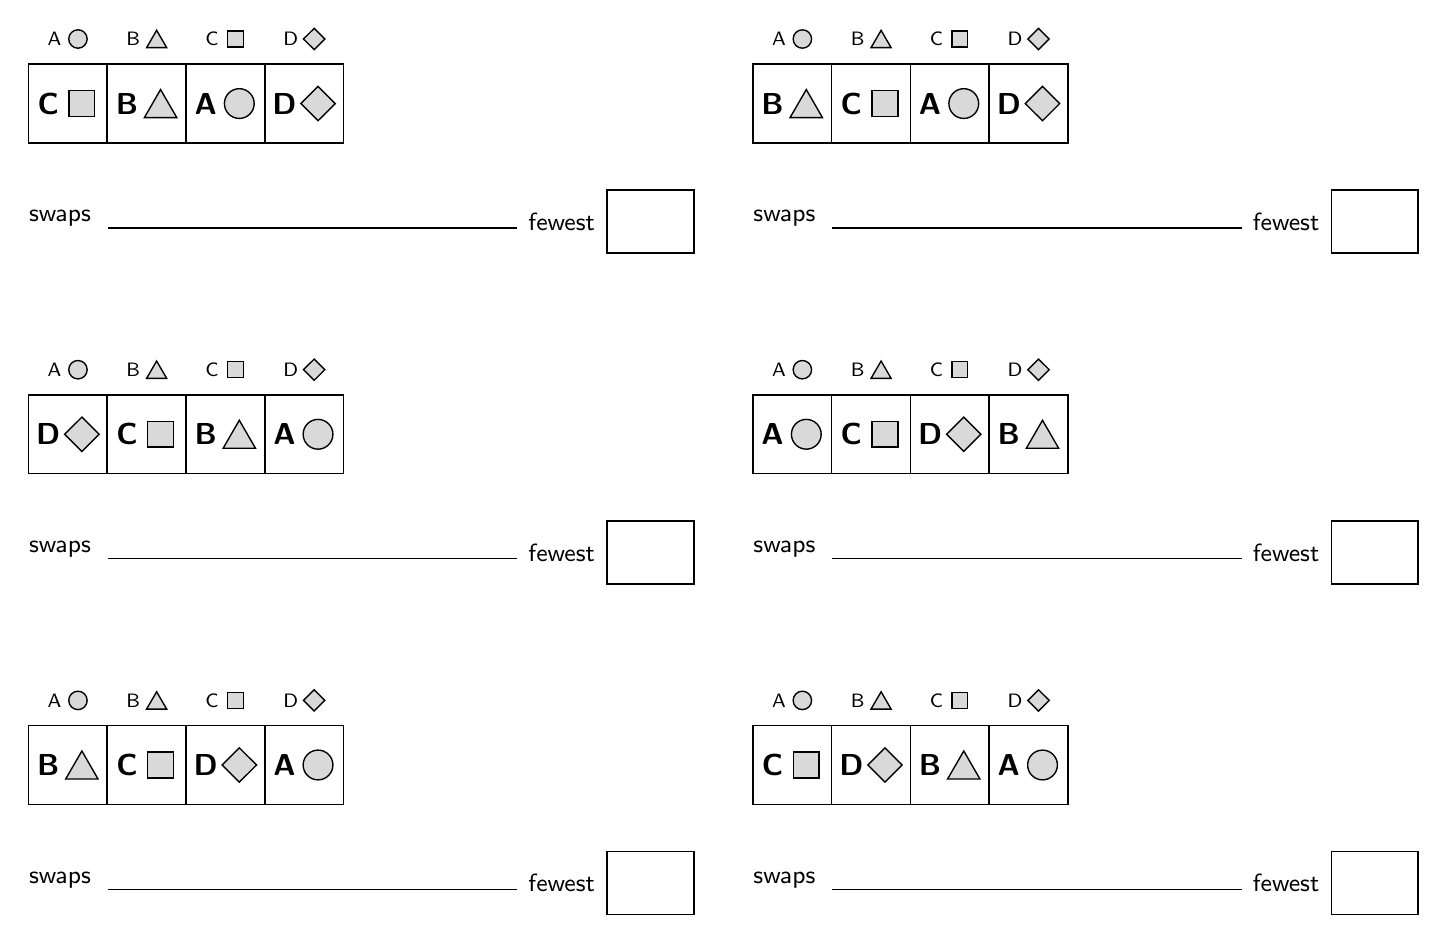
\begin{tikzpicture}[x=1mm, y=1mm]
\draw[line width=0.6pt] (0,0) rectangle (10,10);
\node[inner sep=0, font=\fontsize{7}{8.4}\selectfont] at (3.3,13.2) {A};
\path[fill=gray!30, draw=black, line width=0.5pt] (6.28,13.2) circle (1.17);
\node[inner sep=0, font=\fontsize{11}{13.2}\selectfont\bfseries] at (2.5,5) {C};
\path[fill=gray!30, draw=black, line width=0.5pt] (5.14,3.36) rectangle (8.41,6.64);
\draw[line width=0.6pt] (10,0) rectangle (20,10);
\node[inner sep=0, font=\fontsize{7}{8.4}\selectfont] at (13.3,13.2) {B};
\path[fill=gray!30, draw=black, line width=0.5pt] (16.27,14.3) -- (15,12.1) -- (17.55,12.1) -- cycle;
\node[inner sep=0, font=\fontsize{11}{13.2}\selectfont\bfseries] at (12.5,5) {B};
\path[fill=gray!30, draw=black, line width=0.5pt] (16.77,6.78) -- (14.72,3.22) -- (18.83,3.22) -- cycle;
\draw[line width=0.6pt] (20,0) rectangle (30,10);
\node[inner sep=0, font=\fontsize{7}{8.4}\selectfont] at (23.3,13.2) {C};
\path[fill=gray!30, draw=black, line width=0.5pt] (25.26,12.19) rectangle (27.29,14.21);
\node[inner sep=0, font=\fontsize{11}{13.2}\selectfont\bfseries] at (22.5,5) {A};
\path[fill=gray!30, draw=black, line width=0.5pt] (26.77,5) circle (1.89);
\draw[line width=0.6pt] (30,0) rectangle (40,10);
\node[inner sep=0, font=\fontsize{7}{8.4}\selectfont] at (33.3,13.2) {D};
\path[fill=gray!30, draw=black, line width=0.5pt] (36.28,14.55) -- (37.63,13.2) -- (36.28,11.85) -- (34.92,13.2) -- cycle;
\node[inner sep=0, font=\fontsize{11}{13.2}\selectfont\bfseries] at (32.5,5) {D};
\path[fill=gray!30, draw=black, line width=0.5pt] (36.77,7.18) -- (38.96,5) -- (36.77,2.82) -- (34.59,5) -- cycle;
\node[anchor=base west, inner sep=0, font=\fontsize{9}{10.8}\selectfont] at (0,-10) {swaps};
\draw[line width=0.4pt] (10.05,-10.8) -- (62.05,-10.8);
\node[anchor=east, inner sep=0, font=\fontsize{9}{10.8}\selectfont] at (72,-10) {fewest};
\draw[line width=0.6pt] (73.5,-14) rectangle (84.5,-6);
\draw[line width=0.6pt] (92,0) rectangle (102,10);
\node[inner sep=0, font=\fontsize{7}{8.4}\selectfont] at (95.3,13.2) {A};
\path[fill=gray!30, draw=black, line width=0.5pt] (98.28,13.2) circle (1.17);
\node[inner sep=0, font=\fontsize{11}{13.2}\selectfont\bfseries] at (94.5,5) {B};
\path[fill=gray!30, draw=black, line width=0.5pt] (98.78,6.78) -- (96.72,3.22) -- (100.83,3.22) -- cycle;
\draw[line width=0.6pt] (102,0) rectangle (112,10);
\node[inner sep=0, font=\fontsize{7}{8.4}\selectfont] at (105.3,13.2) {B};
\path[fill=gray!30, draw=black, line width=0.5pt] (108.28,14.3) -- (107,12.1) -- (109.55,12.1) -- cycle;
\node[inner sep=0, font=\fontsize{11}{13.2}\selectfont\bfseries] at (104.5,5) {C};
\path[fill=gray!30, draw=black, line width=0.5pt] (107.14,3.36) rectangle (110.41,6.64);
\draw[line width=0.6pt] (112,0) rectangle (122,10);
\node[inner sep=0, font=\fontsize{7}{8.4}\selectfont] at (115.3,13.2) {C};
\path[fill=gray!30, draw=black, line width=0.5pt] (117.26,12.19) rectangle (119.29,14.21);
\node[inner sep=0, font=\fontsize{11}{13.2}\selectfont\bfseries] at (114.5,5) {A};
\path[fill=gray!30, draw=black, line width=0.5pt] (118.78,5) circle (1.89);
\draw[line width=0.6pt] (122,0) rectangle (132,10);
\node[inner sep=0, font=\fontsize{7}{8.4}\selectfont] at (125.3,13.2) {D};
\path[fill=gray!30, draw=black, line width=0.5pt] (128.27,14.55) -- (129.63,13.2) -- (128.27,11.85) -- (126.92,13.2) -- cycle;
\node[inner sep=0, font=\fontsize{11}{13.2}\selectfont\bfseries] at (124.5,5) {D};
\path[fill=gray!30, draw=black, line width=0.5pt] (128.78,7.18) -- (130.96,5) -- (128.78,2.82) -- (126.59,5) -- cycle;
\node[anchor=base west, inner sep=0, font=\fontsize{9}{10.8}\selectfont] at (92,-10) {swaps};
\draw[line width=0.4pt] (102.05,-10.8) -- (154.05,-10.8);
\node[anchor=east, inner sep=0, font=\fontsize{9}{10.8}\selectfont] at (164,-10) {fewest};
\draw[line width=0.6pt] (165.5,-14) rectangle (176.5,-6);
\draw[line width=0.6pt] (0,-42) rectangle (10,-32);
\node[inner sep=0, font=\fontsize{7}{8.4}\selectfont] at (3.3,-28.8) {A};
\path[fill=gray!30, draw=black, line width=0.5pt] (6.28,-28.8) circle (1.17);
\node[inner sep=0, font=\fontsize{11}{13.2}\selectfont\bfseries] at (2.5,-37) {D};
\path[fill=gray!30, draw=black, line width=0.5pt] (6.78,-34.82) -- (8.96,-37) -- (6.78,-39.18) -- (4.59,-37) -- cycle;
\draw[line width=0.6pt] (10,-42) rectangle (20,-32);
\node[inner sep=0, font=\fontsize{7}{8.4}\selectfont] at (13.3,-28.8) {B};
\path[fill=gray!30, draw=black, line width=0.5pt] (16.27,-27.7) -- (15,-29.9) -- (17.55,-29.9) -- cycle;
\node[inner sep=0, font=\fontsize{11}{13.2}\selectfont\bfseries] at (12.5,-37) {C};
\path[fill=gray!30, draw=black, line width=0.5pt] (15.14,-38.64) rectangle (18.41,-35.36);
\draw[line width=0.6pt] (20,-42) rectangle (30,-32);
\node[inner sep=0, font=\fontsize{7}{8.4}\selectfont] at (23.3,-28.8) {C};
\path[fill=gray!30, draw=black, line width=0.5pt] (25.26,-29.81) rectangle (27.29,-27.79);
\node[inner sep=0, font=\fontsize{11}{13.2}\selectfont\bfseries] at (22.5,-37) {B};
\path[fill=gray!30, draw=black, line width=0.5pt] (26.77,-35.22) -- (24.72,-38.78) -- (28.83,-38.78) -- cycle;
\draw[line width=0.6pt] (30,-42) rectangle (40,-32);
\node[inner sep=0, font=\fontsize{7}{8.4}\selectfont] at (33.3,-28.8) {D};
\path[fill=gray!30, draw=black, line width=0.5pt] (36.28,-27.45) -- (37.63,-28.8) -- (36.28,-30.15) -- (34.92,-28.8) -- cycle;
\node[inner sep=0, font=\fontsize{11}{13.2}\selectfont\bfseries] at (32.5,-37) {A};
\path[fill=gray!30, draw=black, line width=0.5pt] (36.77,-37) circle (1.89);
\node[anchor=base west, inner sep=0, font=\fontsize{9}{10.8}\selectfont] at (0,-52) {swaps};
\draw[line width=0.4pt] (10.05,-52.8) -- (62.05,-52.8);
\node[anchor=east, inner sep=0, font=\fontsize{9}{10.8}\selectfont] at (72,-52) {fewest};
\draw[line width=0.6pt] (73.5,-56) rectangle (84.5,-48);
\draw[line width=0.6pt] (92,-42) rectangle (102,-32);
\node[inner sep=0, font=\fontsize{7}{8.4}\selectfont] at (95.3,-28.8) {A};
\path[fill=gray!30, draw=black, line width=0.5pt] (98.28,-28.8) circle (1.17);
\node[inner sep=0, font=\fontsize{11}{13.2}\selectfont\bfseries] at (94.5,-37) {A};
\path[fill=gray!30, draw=black, line width=0.5pt] (98.78,-37) circle (1.89);
\draw[line width=0.6pt] (102,-42) rectangle (112,-32);
\node[inner sep=0, font=\fontsize{7}{8.4}\selectfont] at (105.3,-28.8) {B};
\path[fill=gray!30, draw=black, line width=0.5pt] (108.28,-27.7) -- (107,-29.9) -- (109.55,-29.9) -- cycle;
\node[inner sep=0, font=\fontsize{11}{13.2}\selectfont\bfseries] at (104.5,-37) {C};
\path[fill=gray!30, draw=black, line width=0.5pt] (107.14,-38.64) rectangle (110.41,-35.36);
\draw[line width=0.6pt] (112,-42) rectangle (122,-32);
\node[inner sep=0, font=\fontsize{7}{8.4}\selectfont] at (115.3,-28.8) {C};
\path[fill=gray!30, draw=black, line width=0.5pt] (117.26,-29.81) rectangle (119.29,-27.79);
\node[inner sep=0, font=\fontsize{11}{13.2}\selectfont\bfseries] at (114.5,-37) {D};
\path[fill=gray!30, draw=black, line width=0.5pt] (118.78,-34.82) -- (120.96,-37) -- (118.78,-39.18) -- (116.59,-37) -- cycle;
\draw[line width=0.6pt] (122,-42) rectangle (132,-32);
\node[inner sep=0, font=\fontsize{7}{8.4}\selectfont] at (125.3,-28.8) {D};
\path[fill=gray!30, draw=black, line width=0.5pt] (128.27,-27.45) -- (129.63,-28.8) -- (128.27,-30.15) -- (126.92,-28.8) -- cycle;
\node[inner sep=0, font=\fontsize{11}{13.2}\selectfont\bfseries] at (124.5,-37) {B};
\path[fill=gray!30, draw=black, line width=0.5pt] (128.78,-35.22) -- (126.72,-38.78) -- (130.83,-38.78) -- cycle;
\node[anchor=base west, inner sep=0, font=\fontsize{9}{10.8}\selectfont] at (92,-52) {swaps};
\draw[line width=0.4pt] (102.05,-52.8) -- (154.05,-52.8);
\node[anchor=east, inner sep=0, font=\fontsize{9}{10.8}\selectfont] at (164,-52) {fewest};
\draw[line width=0.6pt] (165.5,-56) rectangle (176.5,-48);
\draw[line width=0.6pt] (0,-84) rectangle (10,-74);
\node[inner sep=0, font=\fontsize{7}{8.4}\selectfont] at (3.3,-70.8) {A};
\path[fill=gray!30, draw=black, line width=0.5pt] (6.28,-70.8) circle (1.17);
\node[inner sep=0, font=\fontsize{11}{13.2}\selectfont\bfseries] at (2.5,-79) {B};
\path[fill=gray!30, draw=black, line width=0.5pt] (6.78,-77.22) -- (4.72,-80.78) -- (8.83,-80.78) -- cycle;
\draw[line width=0.6pt] (10,-84) rectangle (20,-74);
\node[inner sep=0, font=\fontsize{7}{8.4}\selectfont] at (13.3,-70.8) {B};
\path[fill=gray!30, draw=black, line width=0.5pt] (16.27,-69.7) -- (15,-71.9) -- (17.55,-71.9) -- cycle;
\node[inner sep=0, font=\fontsize{11}{13.2}\selectfont\bfseries] at (12.5,-79) {C};
\path[fill=gray!30, draw=black, line width=0.5pt] (15.14,-80.64) rectangle (18.41,-77.36);
\draw[line width=0.6pt] (20,-84) rectangle (30,-74);
\node[inner sep=0, font=\fontsize{7}{8.4}\selectfont] at (23.3,-70.8) {C};
\path[fill=gray!30, draw=black, line width=0.5pt] (25.26,-71.81) rectangle (27.29,-69.79);
\node[inner sep=0, font=\fontsize{11}{13.2}\selectfont\bfseries] at (22.5,-79) {D};
\path[fill=gray!30, draw=black, line width=0.5pt] (26.77,-76.82) -- (28.96,-79) -- (26.77,-81.18) -- (24.59,-79) -- cycle;
\draw[line width=0.6pt] (30,-84) rectangle (40,-74);
\node[inner sep=0, font=\fontsize{7}{8.4}\selectfont] at (33.3,-70.8) {D};
\path[fill=gray!30, draw=black, line width=0.5pt] (36.28,-69.45) -- (37.63,-70.8) -- (36.28,-72.15) -- (34.92,-70.8) -- cycle;
\node[inner sep=0, font=\fontsize{11}{13.2}\selectfont\bfseries] at (32.5,-79) {A};
\path[fill=gray!30, draw=black, line width=0.5pt] (36.77,-79) circle (1.89);
\node[anchor=base west, inner sep=0, font=\fontsize{9}{10.8}\selectfont] at (0,-94) {swaps};
\draw[line width=0.4pt] (10.05,-94.8) -- (62.05,-94.8);
\node[anchor=east, inner sep=0, font=\fontsize{9}{10.8}\selectfont] at (72,-94) {fewest};
\draw[line width=0.6pt] (73.5,-98) rectangle (84.5,-90);
\draw[line width=0.6pt] (92,-84) rectangle (102,-74);
\node[inner sep=0, font=\fontsize{7}{8.4}\selectfont] at (95.3,-70.8) {A};
\path[fill=gray!30, draw=black, line width=0.5pt] (98.28,-70.8) circle (1.17);
\node[inner sep=0, font=\fontsize{11}{13.2}\selectfont\bfseries] at (94.5,-79) {C};
\path[fill=gray!30, draw=black, line width=0.5pt] (97.14,-80.64) rectangle (100.41,-77.36);
\draw[line width=0.6pt] (102,-84) rectangle (112,-74);
\node[inner sep=0, font=\fontsize{7}{8.4}\selectfont] at (105.3,-70.8) {B};
\path[fill=gray!30, draw=black, line width=0.5pt] (108.28,-69.7) -- (107,-71.9) -- (109.55,-71.9) -- cycle;
\node[inner sep=0, font=\fontsize{11}{13.2}\selectfont\bfseries] at (104.5,-79) {D};
\path[fill=gray!30, draw=black, line width=0.5pt] (108.78,-76.82) -- (110.96,-79) -- (108.78,-81.18) -- (106.59,-79) -- cycle;
\draw[line width=0.6pt] (112,-84) rectangle (122,-74);
\node[inner sep=0, font=\fontsize{7}{8.4}\selectfont] at (115.3,-70.8) {C};
\path[fill=gray!30, draw=black, line width=0.5pt] (117.26,-71.81) rectangle (119.29,-69.79);
\node[inner sep=0, font=\fontsize{11}{13.2}\selectfont\bfseries] at (114.5,-79) {B};
\path[fill=gray!30, draw=black, line width=0.5pt] (118.78,-77.22) -- (116.72,-80.78) -- (120.83,-80.78) -- cycle;
\draw[line width=0.6pt] (122,-84) rectangle (132,-74);
\node[inner sep=0, font=\fontsize{7}{8.4}\selectfont] at (125.3,-70.8) {D};
\path[fill=gray!30, draw=black, line width=0.5pt] (128.27,-69.45) -- (129.63,-70.8) -- (128.27,-72.15) -- (126.92,-70.8) -- cycle;
\node[inner sep=0, font=\fontsize{11}{13.2}\selectfont\bfseries] at (124.5,-79) {A};
\path[fill=gray!30, draw=black, line width=0.5pt] (128.78,-79) circle (1.89);
\node[anchor=base west, inner sep=0, font=\fontsize{9}{10.8}\selectfont] at (92,-94) {swaps};
\draw[line width=0.4pt] (102.05,-94.8) -- (154.05,-94.8);
\node[anchor=east, inner sep=0, font=\fontsize{9}{10.8}\selectfont] at (164,-94) {fewest};
\draw[line width=0.6pt] (165.5,-98) rectangle (176.5,-90);
\end{tikzpicture}\par

\vspace{10mm}
\prob{3} Find every row of A, B, C and D that needs the most swaps to come home. Could any row need 4 swaps? Explain.

\par\vspace{3mm}\noindent\hspace*{2mm}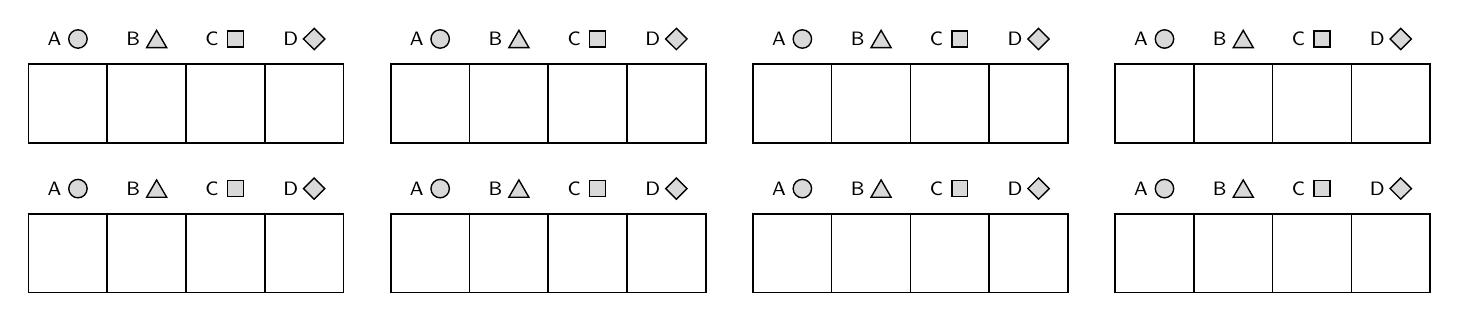
\begin{tikzpicture}[x=1mm, y=1mm]
\draw[line width=0.6pt] (0,0) rectangle (10,10);
\node[inner sep=0, font=\fontsize{7}{8.4}\selectfont] at (3.3,13.2) {A};
\path[fill=gray!30, draw=black, line width=0.5pt] (6.28,13.2) circle (1.17);
\draw[line width=0.6pt] (10,0) rectangle (20,10);
\node[inner sep=0, font=\fontsize{7}{8.4}\selectfont] at (13.3,13.2) {B};
\path[fill=gray!30, draw=black, line width=0.5pt] (16.27,14.3) -- (15,12.1) -- (17.55,12.1) -- cycle;
\draw[line width=0.6pt] (20,0) rectangle (30,10);
\node[inner sep=0, font=\fontsize{7}{8.4}\selectfont] at (23.3,13.2) {C};
\path[fill=gray!30, draw=black, line width=0.5pt] (25.26,12.19) rectangle (27.29,14.21);
\draw[line width=0.6pt] (30,0) rectangle (40,10);
\node[inner sep=0, font=\fontsize{7}{8.4}\selectfont] at (33.3,13.2) {D};
\path[fill=gray!30, draw=black, line width=0.5pt] (36.28,14.55) -- (37.63,13.2) -- (36.28,11.85) -- (34.92,13.2) -- cycle;
\draw[line width=0.6pt] (46,0) rectangle (56,10);
\node[inner sep=0, font=\fontsize{7}{8.4}\selectfont] at (49.3,13.2) {A};
\path[fill=gray!30, draw=black, line width=0.5pt] (52.28,13.2) circle (1.17);
\draw[line width=0.6pt] (56,0) rectangle (66,10);
\node[inner sep=0, font=\fontsize{7}{8.4}\selectfont] at (59.3,13.2) {B};
\path[fill=gray!30, draw=black, line width=0.5pt] (62.28,14.3) -- (61,12.1) -- (63.55,12.1) -- cycle;
\draw[line width=0.6pt] (66,0) rectangle (76,10);
\node[inner sep=0, font=\fontsize{7}{8.4}\selectfont] at (69.3,13.2) {C};
\path[fill=gray!30, draw=black, line width=0.5pt] (71.26,12.19) rectangle (73.29,14.21);
\draw[line width=0.6pt] (76,0) rectangle (86,10);
\node[inner sep=0, font=\fontsize{7}{8.4}\selectfont] at (79.3,13.2) {D};
\path[fill=gray!30, draw=black, line width=0.5pt] (82.28,14.55) -- (83.63,13.2) -- (82.28,11.85) -- (80.92,13.2) -- cycle;
\draw[line width=0.6pt] (92,0) rectangle (102,10);
\node[inner sep=0, font=\fontsize{7}{8.4}\selectfont] at (95.3,13.2) {A};
\path[fill=gray!30, draw=black, line width=0.5pt] (98.28,13.2) circle (1.17);
\draw[line width=0.6pt] (102,0) rectangle (112,10);
\node[inner sep=0, font=\fontsize{7}{8.4}\selectfont] at (105.3,13.2) {B};
\path[fill=gray!30, draw=black, line width=0.5pt] (108.28,14.3) -- (107,12.1) -- (109.55,12.1) -- cycle;
\draw[line width=0.6pt] (112,0) rectangle (122,10);
\node[inner sep=0, font=\fontsize{7}{8.4}\selectfont] at (115.3,13.2) {C};
\path[fill=gray!30, draw=black, line width=0.5pt] (117.26,12.19) rectangle (119.29,14.21);
\draw[line width=0.6pt] (122,0) rectangle (132,10);
\node[inner sep=0, font=\fontsize{7}{8.4}\selectfont] at (125.3,13.2) {D};
\path[fill=gray!30, draw=black, line width=0.5pt] (128.27,14.55) -- (129.63,13.2) -- (128.27,11.85) -- (126.92,13.2) -- cycle;
\draw[line width=0.6pt] (138,0) rectangle (148,10);
\node[inner sep=0, font=\fontsize{7}{8.4}\selectfont] at (141.3,13.2) {A};
\path[fill=gray!30, draw=black, line width=0.5pt] (144.27,13.2) circle (1.17);
\draw[line width=0.6pt] (148,0) rectangle (158,10);
\node[inner sep=0, font=\fontsize{7}{8.4}\selectfont] at (151.3,13.2) {B};
\path[fill=gray!30, draw=black, line width=0.5pt] (154.27,14.3) -- (153,12.1) -- (155.55,12.1) -- cycle;
\draw[line width=0.6pt] (158,0) rectangle (168,10);
\node[inner sep=0, font=\fontsize{7}{8.4}\selectfont] at (161.3,13.2) {C};
\path[fill=gray!30, draw=black, line width=0.5pt] (163.26,12.19) rectangle (165.29,14.21);
\draw[line width=0.6pt] (168,0) rectangle (178,10);
\node[inner sep=0, font=\fontsize{7}{8.4}\selectfont] at (171.3,13.2) {D};
\path[fill=gray!30, draw=black, line width=0.5pt] (174.27,14.55) -- (175.63,13.2) -- (174.27,11.85) -- (172.92,13.2) -- cycle;
\draw[line width=0.6pt] (0,-19) rectangle (10,-9);
\node[inner sep=0, font=\fontsize{7}{8.4}\selectfont] at (3.3,-5.8) {A};
\path[fill=gray!30, draw=black, line width=0.5pt] (6.28,-5.8) circle (1.17);
\draw[line width=0.6pt] (10,-19) rectangle (20,-9);
\node[inner sep=0, font=\fontsize{7}{8.4}\selectfont] at (13.3,-5.8) {B};
\path[fill=gray!30, draw=black, line width=0.5pt] (16.27,-4.7) -- (15,-6.9) -- (17.55,-6.9) -- cycle;
\draw[line width=0.6pt] (20,-19) rectangle (30,-9);
\node[inner sep=0, font=\fontsize{7}{8.4}\selectfont] at (23.3,-5.8) {C};
\path[fill=gray!30, draw=black, line width=0.5pt] (25.26,-6.81) rectangle (27.29,-4.79);
\draw[line width=0.6pt] (30,-19) rectangle (40,-9);
\node[inner sep=0, font=\fontsize{7}{8.4}\selectfont] at (33.3,-5.8) {D};
\path[fill=gray!30, draw=black, line width=0.5pt] (36.28,-4.45) -- (37.63,-5.8) -- (36.28,-7.15) -- (34.92,-5.8) -- cycle;
\draw[line width=0.6pt] (46,-19) rectangle (56,-9);
\node[inner sep=0, font=\fontsize{7}{8.4}\selectfont] at (49.3,-5.8) {A};
\path[fill=gray!30, draw=black, line width=0.5pt] (52.28,-5.8) circle (1.17);
\draw[line width=0.6pt] (56,-19) rectangle (66,-9);
\node[inner sep=0, font=\fontsize{7}{8.4}\selectfont] at (59.3,-5.8) {B};
\path[fill=gray!30, draw=black, line width=0.5pt] (62.28,-4.7) -- (61,-6.9) -- (63.55,-6.9) -- cycle;
\draw[line width=0.6pt] (66,-19) rectangle (76,-9);
\node[inner sep=0, font=\fontsize{7}{8.4}\selectfont] at (69.3,-5.8) {C};
\path[fill=gray!30, draw=black, line width=0.5pt] (71.26,-6.81) rectangle (73.29,-4.79);
\draw[line width=0.6pt] (76,-19) rectangle (86,-9);
\node[inner sep=0, font=\fontsize{7}{8.4}\selectfont] at (79.3,-5.8) {D};
\path[fill=gray!30, draw=black, line width=0.5pt] (82.28,-4.45) -- (83.63,-5.8) -- (82.28,-7.15) -- (80.92,-5.8) -- cycle;
\draw[line width=0.6pt] (92,-19) rectangle (102,-9);
\node[inner sep=0, font=\fontsize{7}{8.4}\selectfont] at (95.3,-5.8) {A};
\path[fill=gray!30, draw=black, line width=0.5pt] (98.28,-5.8) circle (1.17);
\draw[line width=0.6pt] (102,-19) rectangle (112,-9);
\node[inner sep=0, font=\fontsize{7}{8.4}\selectfont] at (105.3,-5.8) {B};
\path[fill=gray!30, draw=black, line width=0.5pt] (108.28,-4.7) -- (107,-6.9) -- (109.55,-6.9) -- cycle;
\draw[line width=0.6pt] (112,-19) rectangle (122,-9);
\node[inner sep=0, font=\fontsize{7}{8.4}\selectfont] at (115.3,-5.8) {C};
\path[fill=gray!30, draw=black, line width=0.5pt] (117.26,-6.81) rectangle (119.29,-4.79);
\draw[line width=0.6pt] (122,-19) rectangle (132,-9);
\node[inner sep=0, font=\fontsize{7}{8.4}\selectfont] at (125.3,-5.8) {D};
\path[fill=gray!30, draw=black, line width=0.5pt] (128.27,-4.45) -- (129.63,-5.8) -- (128.27,-7.15) -- (126.92,-5.8) -- cycle;
\draw[line width=0.6pt] (138,-19) rectangle (148,-9);
\node[inner sep=0, font=\fontsize{7}{8.4}\selectfont] at (141.3,-5.8) {A};
\path[fill=gray!30, draw=black, line width=0.5pt] (144.27,-5.8) circle (1.17);
\draw[line width=0.6pt] (148,-19) rectangle (158,-9);
\node[inner sep=0, font=\fontsize{7}{8.4}\selectfont] at (151.3,-5.8) {B};
\path[fill=gray!30, draw=black, line width=0.5pt] (154.27,-4.7) -- (153,-6.9) -- (155.55,-6.9) -- cycle;
\draw[line width=0.6pt] (158,-19) rectangle (168,-9);
\node[inner sep=0, font=\fontsize{7}{8.4}\selectfont] at (161.3,-5.8) {C};
\path[fill=gray!30, draw=black, line width=0.5pt] (163.26,-6.81) rectangle (165.29,-4.79);
\draw[line width=0.6pt] (168,-19) rectangle (178,-9);
\node[inner sep=0, font=\fontsize{7}{8.4}\selectfont] at (171.3,-5.8) {D};
\path[fill=gray!30, draw=black, line width=0.5pt] (174.27,-4.45) -- (175.63,-5.8) -- (174.27,-7.15) -- (172.92,-5.8) -- cycle;
\end{tikzpicture}\par

\vfill
\newpage
\prob{4} In which of these rows can one swap bring two cards home at once? Explain how you can tell for any row.

\par\vspace{3mm}\noindent\hspace*{2mm}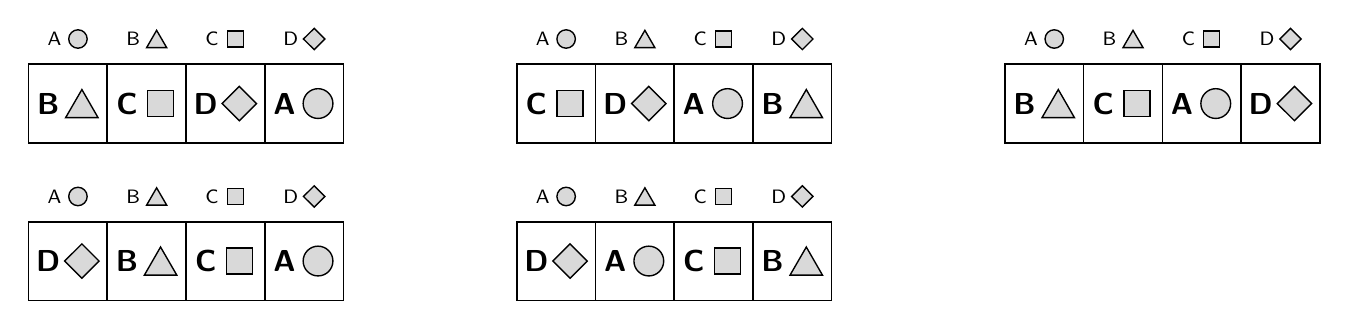
\begin{tikzpicture}[x=1mm, y=1mm]
\draw[line width=0.6pt] (0,0) rectangle (10,10);
\node[inner sep=0, font=\fontsize{7}{8.4}\selectfont] at (3.3,13.2) {A};
\path[fill=gray!30, draw=black, line width=0.5pt] (6.28,13.2) circle (1.17);
\node[inner sep=0, font=\fontsize{11}{13.2}\selectfont\bfseries] at (2.5,5) {B};
\path[fill=gray!30, draw=black, line width=0.5pt] (6.78,6.78) -- (4.72,3.22) -- (8.83,3.22) -- cycle;
\draw[line width=0.6pt] (10,0) rectangle (20,10);
\node[inner sep=0, font=\fontsize{7}{8.4}\selectfont] at (13.3,13.2) {B};
\path[fill=gray!30, draw=black, line width=0.5pt] (16.27,14.3) -- (15,12.1) -- (17.55,12.1) -- cycle;
\node[inner sep=0, font=\fontsize{11}{13.2}\selectfont\bfseries] at (12.5,5) {C};
\path[fill=gray!30, draw=black, line width=0.5pt] (15.14,3.36) rectangle (18.41,6.64);
\draw[line width=0.6pt] (20,0) rectangle (30,10);
\node[inner sep=0, font=\fontsize{7}{8.4}\selectfont] at (23.3,13.2) {C};
\path[fill=gray!30, draw=black, line width=0.5pt] (25.26,12.19) rectangle (27.29,14.21);
\node[inner sep=0, font=\fontsize{11}{13.2}\selectfont\bfseries] at (22.5,5) {D};
\path[fill=gray!30, draw=black, line width=0.5pt] (26.77,7.18) -- (28.96,5) -- (26.77,2.82) -- (24.59,5) -- cycle;
\draw[line width=0.6pt] (30,0) rectangle (40,10);
\node[inner sep=0, font=\fontsize{7}{8.4}\selectfont] at (33.3,13.2) {D};
\path[fill=gray!30, draw=black, line width=0.5pt] (36.28,14.55) -- (37.63,13.2) -- (36.28,11.85) -- (34.92,13.2) -- cycle;
\node[inner sep=0, font=\fontsize{11}{13.2}\selectfont\bfseries] at (32.5,5) {A};
\path[fill=gray!30, draw=black, line width=0.5pt] (36.77,5) circle (1.89);
\draw[line width=0.6pt] (62,0) rectangle (72,10);
\node[inner sep=0, font=\fontsize{7}{8.4}\selectfont] at (65.3,13.2) {A};
\path[fill=gray!30, draw=black, line width=0.5pt] (68.28,13.2) circle (1.17);
\node[inner sep=0, font=\fontsize{11}{13.2}\selectfont\bfseries] at (64.5,5) {C};
\path[fill=gray!30, draw=black, line width=0.5pt] (67.14,3.36) rectangle (70.41,6.64);
\draw[line width=0.6pt] (72,0) rectangle (82,10);
\node[inner sep=0, font=\fontsize{7}{8.4}\selectfont] at (75.3,13.2) {B};
\path[fill=gray!30, draw=black, line width=0.5pt] (78.28,14.3) -- (77,12.1) -- (79.55,12.1) -- cycle;
\node[inner sep=0, font=\fontsize{11}{13.2}\selectfont\bfseries] at (74.5,5) {D};
\path[fill=gray!30, draw=black, line width=0.5pt] (78.78,7.18) -- (80.96,5) -- (78.78,2.82) -- (76.59,5) -- cycle;
\draw[line width=0.6pt] (82,0) rectangle (92,10);
\node[inner sep=0, font=\fontsize{7}{8.4}\selectfont] at (85.3,13.2) {C};
\path[fill=gray!30, draw=black, line width=0.5pt] (87.26,12.19) rectangle (89.29,14.21);
\node[inner sep=0, font=\fontsize{11}{13.2}\selectfont\bfseries] at (84.5,5) {A};
\path[fill=gray!30, draw=black, line width=0.5pt] (88.78,5) circle (1.89);
\draw[line width=0.6pt] (92,0) rectangle (102,10);
\node[inner sep=0, font=\fontsize{7}{8.4}\selectfont] at (95.3,13.2) {D};
\path[fill=gray!30, draw=black, line width=0.5pt] (98.28,14.55) -- (99.63,13.2) -- (98.28,11.85) -- (96.92,13.2) -- cycle;
\node[inner sep=0, font=\fontsize{11}{13.2}\selectfont\bfseries] at (94.5,5) {B};
\path[fill=gray!30, draw=black, line width=0.5pt] (98.78,6.78) -- (96.72,3.22) -- (100.83,3.22) -- cycle;
\draw[line width=0.6pt] (124,0) rectangle (134,10);
\node[inner sep=0, font=\fontsize{7}{8.4}\selectfont] at (127.3,13.2) {A};
\path[fill=gray!30, draw=black, line width=0.5pt] (130.27,13.2) circle (1.17);
\node[inner sep=0, font=\fontsize{11}{13.2}\selectfont\bfseries] at (126.5,5) {B};
\path[fill=gray!30, draw=black, line width=0.5pt] (130.78,6.78) -- (128.72,3.22) -- (132.83,3.22) -- cycle;
\draw[line width=0.6pt] (134,0) rectangle (144,10);
\node[inner sep=0, font=\fontsize{7}{8.4}\selectfont] at (137.3,13.2) {B};
\path[fill=gray!30, draw=black, line width=0.5pt] (140.27,14.3) -- (139,12.1) -- (141.55,12.1) -- cycle;
\node[inner sep=0, font=\fontsize{11}{13.2}\selectfont\bfseries] at (136.5,5) {C};
\path[fill=gray!30, draw=black, line width=0.5pt] (139.14,3.36) rectangle (142.41,6.64);
\draw[line width=0.6pt] (144,0) rectangle (154,10);
\node[inner sep=0, font=\fontsize{7}{8.4}\selectfont] at (147.3,13.2) {C};
\path[fill=gray!30, draw=black, line width=0.5pt] (149.26,12.19) rectangle (151.29,14.21);
\node[inner sep=0, font=\fontsize{11}{13.2}\selectfont\bfseries] at (146.5,5) {A};
\path[fill=gray!30, draw=black, line width=0.5pt] (150.78,5) circle (1.89);
\draw[line width=0.6pt] (154,0) rectangle (164,10);
\node[inner sep=0, font=\fontsize{7}{8.4}\selectfont] at (157.3,13.2) {D};
\path[fill=gray!30, draw=black, line width=0.5pt] (160.27,14.55) -- (161.63,13.2) -- (160.27,11.85) -- (158.92,13.2) -- cycle;
\node[inner sep=0, font=\fontsize{11}{13.2}\selectfont\bfseries] at (156.5,5) {D};
\path[fill=gray!30, draw=black, line width=0.5pt] (160.78,7.18) -- (162.96,5) -- (160.78,2.82) -- (158.59,5) -- cycle;
\draw[line width=0.6pt] (0,-20) rectangle (10,-10);
\node[inner sep=0, font=\fontsize{7}{8.4}\selectfont] at (3.3,-6.8) {A};
\path[fill=gray!30, draw=black, line width=0.5pt] (6.28,-6.8) circle (1.17);
\node[inner sep=0, font=\fontsize{11}{13.2}\selectfont\bfseries] at (2.5,-15) {D};
\path[fill=gray!30, draw=black, line width=0.5pt] (6.78,-12.82) -- (8.96,-15) -- (6.78,-17.18) -- (4.59,-15) -- cycle;
\draw[line width=0.6pt] (10,-20) rectangle (20,-10);
\node[inner sep=0, font=\fontsize{7}{8.4}\selectfont] at (13.3,-6.8) {B};
\path[fill=gray!30, draw=black, line width=0.5pt] (16.27,-5.7) -- (15,-7.9) -- (17.55,-7.9) -- cycle;
\node[inner sep=0, font=\fontsize{11}{13.2}\selectfont\bfseries] at (12.5,-15) {B};
\path[fill=gray!30, draw=black, line width=0.5pt] (16.77,-13.22) -- (14.72,-16.78) -- (18.83,-16.78) -- cycle;
\draw[line width=0.6pt] (20,-20) rectangle (30,-10);
\node[inner sep=0, font=\fontsize{7}{8.4}\selectfont] at (23.3,-6.8) {C};
\path[fill=gray!30, draw=black, line width=0.5pt] (25.26,-7.81) rectangle (27.29,-5.79);
\node[inner sep=0, font=\fontsize{11}{13.2}\selectfont\bfseries] at (22.5,-15) {C};
\path[fill=gray!30, draw=black, line width=0.5pt] (25.14,-16.64) rectangle (28.41,-13.36);
\draw[line width=0.6pt] (30,-20) rectangle (40,-10);
\node[inner sep=0, font=\fontsize{7}{8.4}\selectfont] at (33.3,-6.8) {D};
\path[fill=gray!30, draw=black, line width=0.5pt] (36.28,-5.45) -- (37.63,-6.8) -- (36.28,-8.15) -- (34.92,-6.8) -- cycle;
\node[inner sep=0, font=\fontsize{11}{13.2}\selectfont\bfseries] at (32.5,-15) {A};
\path[fill=gray!30, draw=black, line width=0.5pt] (36.77,-15) circle (1.89);
\draw[line width=0.6pt] (62,-20) rectangle (72,-10);
\node[inner sep=0, font=\fontsize{7}{8.4}\selectfont] at (65.3,-6.8) {A};
\path[fill=gray!30, draw=black, line width=0.5pt] (68.28,-6.8) circle (1.17);
\node[inner sep=0, font=\fontsize{11}{13.2}\selectfont\bfseries] at (64.5,-15) {D};
\path[fill=gray!30, draw=black, line width=0.5pt] (68.78,-12.82) -- (70.96,-15) -- (68.78,-17.18) -- (66.59,-15) -- cycle;
\draw[line width=0.6pt] (72,-20) rectangle (82,-10);
\node[inner sep=0, font=\fontsize{7}{8.4}\selectfont] at (75.3,-6.8) {B};
\path[fill=gray!30, draw=black, line width=0.5pt] (78.28,-5.7) -- (77,-7.9) -- (79.55,-7.9) -- cycle;
\node[inner sep=0, font=\fontsize{11}{13.2}\selectfont\bfseries] at (74.5,-15) {A};
\path[fill=gray!30, draw=black, line width=0.5pt] (78.78,-15) circle (1.89);
\draw[line width=0.6pt] (82,-20) rectangle (92,-10);
\node[inner sep=0, font=\fontsize{7}{8.4}\selectfont] at (85.3,-6.8) {C};
\path[fill=gray!30, draw=black, line width=0.5pt] (87.26,-7.81) rectangle (89.29,-5.79);
\node[inner sep=0, font=\fontsize{11}{13.2}\selectfont\bfseries] at (84.5,-15) {C};
\path[fill=gray!30, draw=black, line width=0.5pt] (87.14,-16.64) rectangle (90.41,-13.36);
\draw[line width=0.6pt] (92,-20) rectangle (102,-10);
\node[inner sep=0, font=\fontsize{7}{8.4}\selectfont] at (95.3,-6.8) {D};
\path[fill=gray!30, draw=black, line width=0.5pt] (98.28,-5.45) -- (99.63,-6.8) -- (98.28,-8.15) -- (96.92,-6.8) -- cycle;
\node[inner sep=0, font=\fontsize{11}{13.2}\selectfont\bfseries] at (94.5,-15) {B};
\path[fill=gray!30, draw=black, line width=0.5pt] (98.78,-13.22) -- (96.72,-16.78) -- (100.83,-16.78) -- cycle;
\end{tikzpicture}\par

\vspace{56mm}
\prob{5} On the uncut sheet of 24 A--D outcome cards, circle every letter that sits in its own home. How many circles are there in all? How many does each letter get?

\par\vspace{3mm}\noindent\hspace*{2mm}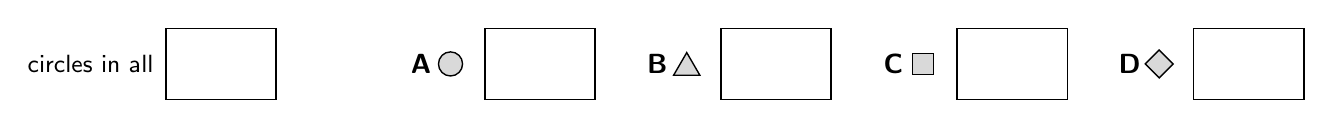
\begin{tikzpicture}[x=1mm, y=1mm]
\node[anchor=east, inner sep=0, font=\fontsize{9}{10.8}\selectfont] at (26,4.5) {circles in all};
\draw[line width=0.6pt] (27.5,0) rectangle (41.5,9);
\node[inner sep=0, font=\fontsize{10}{12.0}\selectfont\bfseries] at (59.9,4.5) {A};
\path[fill=gray!30, draw=black, line width=0.5pt] (63.65,4.5) circle (1.53);
\draw[line width=0.6pt] (68,0) rectangle (82,9);
\node[inner sep=0, font=\fontsize{10}{12.0}\selectfont\bfseries] at (89.9,4.5) {B};
\path[fill=gray!30, draw=black, line width=0.5pt] (93.65,5.94) -- (91.98,3.06) -- (95.32,3.06) -- cycle;
\draw[line width=0.6pt] (98,0) rectangle (112,9);
\node[inner sep=0, font=\fontsize{10}{12.0}\selectfont\bfseries] at (119.9,4.5) {C};
\path[fill=gray!30, draw=black, line width=0.5pt] (122.32,3.17) rectangle (124.98,5.83);
\draw[line width=0.6pt] (128,0) rectangle (142,9);
\node[inner sep=0, font=\fontsize{10}{12.0}\selectfont\bfseries] at (149.9,4.5) {D};
\path[fill=gray!30, draw=black, line width=0.5pt] (153.65,6.27) -- (155.42,4.5) -- (153.65,2.73) -- (151.88,4.5) -- cycle;
\draw[line width=0.6pt] (158,0) rectangle (172,9);
\end{tikzpicture}\par

\vfill
\newpage
\prob{6} How many circles would the six A--C outcome cards get? There are 120 rows of the five cards A, B, C, D and E. How many circles would all 120 rows get? Explain without listing the rows.

\par\vspace{3mm}\noindent\hspace*{0mm}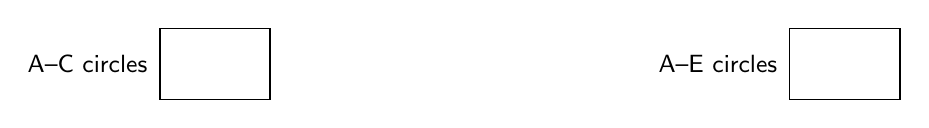
\begin{tikzpicture}[x=1mm, y=1mm]
\node[anchor=east, inner sep=0, font=\fontsize{9}{10.8}\selectfont] at (40,4.5) {A--C circles};
\draw[line width=0.6pt] (41.5,0) rectangle (55.5,9);
\node[anchor=east, inner sep=0, font=\fontsize{9}{10.8}\selectfont] at (120,4.5) {A--E circles};
\draw[line width=0.6pt] (121.5,0) rectangle (135.5,9);
\end{tikzpicture}\par

\vspace{68mm}
\prob{7} Sort the 24 cut A--D outcome cards into piles by how many letters are at home. Explain why the pile with exactly one letter at home and the pile with exactly two have the sizes they do.

\par\vspace{3mm}\noindent\hspace*{4mm}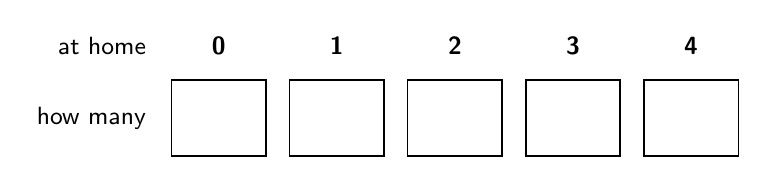
\begin{tikzpicture}[x=1mm, y=1mm]
\node[anchor=east, font=\fontsize{9}{10.8}\selectfont] at (30,14) {at home};
\node[anchor=east, font=\fontsize{9}{10.8}\selectfont] at (30,4.8) {how many};
\node[font=\fontsize{9}{10.8}\selectfont\bfseries] at (38,14) {0};
\draw[line width=0.6pt] (32,0) rectangle (44,9.6);
\node[font=\fontsize{9}{10.8}\selectfont\bfseries] at (53,14) {1};
\draw[line width=0.6pt] (47,0) rectangle (59,9.6);
\node[font=\fontsize{9}{10.8}\selectfont\bfseries] at (68,14) {2};
\draw[line width=0.6pt] (62,0) rectangle (74,9.6);
\node[font=\fontsize{9}{10.8}\selectfont\bfseries] at (83,14) {3};
\draw[line width=0.6pt] (77,0) rectangle (89,9.6);
\node[font=\fontsize{9}{10.8}\selectfont\bfseries] at (98,14) {4};
\draw[line width=0.6pt] (92,0) rectangle (104,9.6);
\end{tikzpicture}\par

\vfill
\newpage
\prob{8} A crossed-out card above a home may not sit in that home. How many of the 24 A--D outcome cards obey each board?

\par\vspace{3mm}\noindent\hspace*{2mm}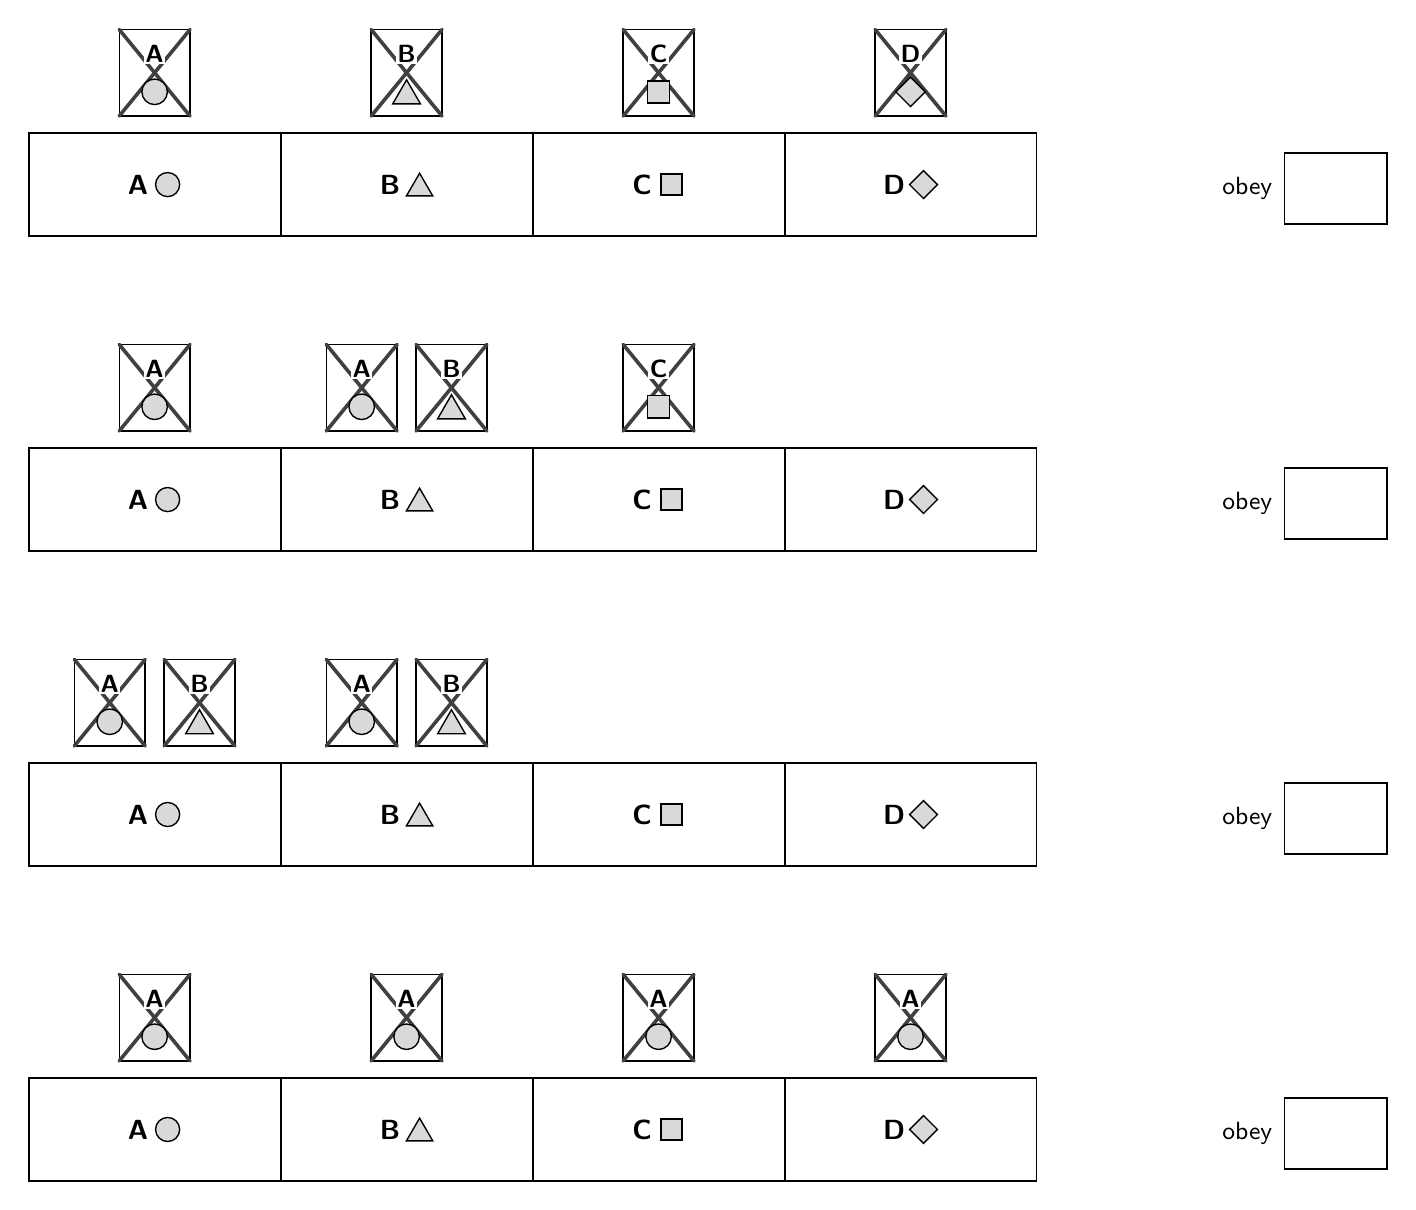
\begin{tikzpicture}[x=1mm, y=1mm]
\draw[line width=0.7pt] (0,0) rectangle (32,13);
\node[inner sep=0, font=\fontsize{10}{12.0}\selectfont\bfseries] at (13.9,6.5) {A};
\path[fill=gray!30, draw=black, line width=0.5pt] (17.65,6.5) circle (1.53);
\draw[line width=0.5pt, draw=black, fill=white] (11.5,15.2) rectangle (20.5,26.2);
\draw[line width=1.3pt, draw=black!75, line cap=round] (11.5,15.2) -- (20.5,26.2);
\draw[line width=1.3pt, draw=black!75, line cap=round] (11.5,26.2) -- (20.5,15.2);
\node[inner sep=0.5pt, fill=white, text=black, font=\fontsize{9}{10.8}\selectfont\bfseries] at (16,23.12) {A};
\path[fill=gray!30, draw=black, line width=0.5pt] (16,18.28) circle (1.62);
\draw[line width=0.7pt] (32,0) rectangle (64,13);
\node[inner sep=0, font=\fontsize{10}{12.0}\selectfont\bfseries] at (45.9,6.5) {B};
\path[fill=gray!30, draw=black, line width=0.5pt] (49.65,7.94) -- (47.98,5.06) -- (51.32,5.06) -- cycle;
\draw[line width=0.5pt, draw=black, fill=white] (43.5,15.2) rectangle (52.5,26.2);
\draw[line width=1.3pt, draw=black!75, line cap=round] (43.5,15.2) -- (52.5,26.2);
\draw[line width=1.3pt, draw=black!75, line cap=round] (43.5,26.2) -- (52.5,15.2);
\node[inner sep=0.5pt, fill=white, text=black, font=\fontsize{9}{10.8}\selectfont\bfseries] at (48,23.12) {B};
\path[fill=gray!30, draw=black, line width=0.5pt] (48,19.81) -- (46.24,16.75) -- (49.76,16.75) -- cycle;
\draw[line width=0.7pt] (64,0) rectangle (96,13);
\node[inner sep=0, font=\fontsize{10}{12.0}\selectfont\bfseries] at (77.9,6.5) {C};
\path[fill=gray!30, draw=black, line width=0.5pt] (80.32,5.17) rectangle (82.98,7.83);
\draw[line width=0.5pt, draw=black, fill=white] (75.5,15.2) rectangle (84.5,26.2);
\draw[line width=1.3pt, draw=black!75, line cap=round] (75.5,15.2) -- (84.5,26.2);
\draw[line width=1.3pt, draw=black!75, line cap=round] (75.5,26.2) -- (84.5,15.2);
\node[inner sep=0.5pt, fill=white, text=black, font=\fontsize{9}{10.8}\selectfont\bfseries] at (80,23.12) {C};
\path[fill=gray!30, draw=black, line width=0.5pt] (78.6,16.88) rectangle (81.4,19.68);
\draw[line width=0.7pt] (96,0) rectangle (128,13);
\node[inner sep=0, font=\fontsize{10}{12.0}\selectfont\bfseries] at (109.9,6.5) {D};
\path[fill=gray!30, draw=black, line width=0.5pt] (113.65,8.27) -- (115.42,6.5) -- (113.65,4.73) -- (111.88,6.5) -- cycle;
\draw[line width=0.5pt, draw=black, fill=white] (107.5,15.2) rectangle (116.5,26.2);
\draw[line width=1.3pt, draw=black!75, line cap=round] (107.5,15.2) -- (116.5,26.2);
\draw[line width=1.3pt, draw=black!75, line cap=round] (107.5,26.2) -- (116.5,15.2);
\node[inner sep=0.5pt, fill=white, text=black, font=\fontsize{9}{10.8}\selectfont\bfseries] at (112,23.12) {D};
\path[fill=gray!30, draw=black, line width=0.5pt] (112,20.15) -- (113.87,18.28) -- (112,16.41) -- (110.13,18.28) -- cycle;
\node[anchor=east, inner sep=0, font=\fontsize{9}{10.8}\selectfont] at (158,6) {obey};
\draw[line width=0.6pt] (159.5,1.5) rectangle (172.5,10.5);
\draw[line width=0.7pt] (0,-40) rectangle (32,-27);
\node[inner sep=0, font=\fontsize{10}{12.0}\selectfont\bfseries] at (13.9,-33.5) {A};
\path[fill=gray!30, draw=black, line width=0.5pt] (17.65,-33.5) circle (1.53);
\draw[line width=0.5pt, draw=black, fill=white] (11.5,-24.8) rectangle (20.5,-13.8);
\draw[line width=1.3pt, draw=black!75, line cap=round] (11.5,-24.8) -- (20.5,-13.8);
\draw[line width=1.3pt, draw=black!75, line cap=round] (11.5,-13.8) -- (20.5,-24.8);
\node[inner sep=0.5pt, fill=white, text=black, font=\fontsize{9}{10.8}\selectfont\bfseries] at (16,-16.88) {A};
\path[fill=gray!30, draw=black, line width=0.5pt] (16,-21.72) circle (1.62);
\draw[line width=0.7pt] (32,-40) rectangle (64,-27);
\node[inner sep=0, font=\fontsize{10}{12.0}\selectfont\bfseries] at (45.9,-33.5) {B};
\path[fill=gray!30, draw=black, line width=0.5pt] (49.65,-32.06) -- (47.98,-34.94) -- (51.32,-34.94) -- cycle;
\draw[line width=0.5pt, draw=black, fill=white] (37.8,-24.8) rectangle (46.8,-13.8);
\draw[line width=1.3pt, draw=black!75, line cap=round] (37.8,-24.8) -- (46.8,-13.8);
\draw[line width=1.3pt, draw=black!75, line cap=round] (37.8,-13.8) -- (46.8,-24.8);
\node[inner sep=0.5pt, fill=white, text=black, font=\fontsize{9}{10.8}\selectfont\bfseries] at (42.3,-16.88) {A};
\path[fill=gray!30, draw=black, line width=0.5pt] (42.3,-21.72) circle (1.62);
\draw[line width=0.5pt, draw=black, fill=white] (49.2,-24.8) rectangle (58.2,-13.8);
\draw[line width=1.3pt, draw=black!75, line cap=round] (49.2,-24.8) -- (58.2,-13.8);
\draw[line width=1.3pt, draw=black!75, line cap=round] (49.2,-13.8) -- (58.2,-24.8);
\node[inner sep=0.5pt, fill=white, text=black, font=\fontsize{9}{10.8}\selectfont\bfseries] at (53.7,-16.88) {B};
\path[fill=gray!30, draw=black, line width=0.5pt] (53.7,-20.19) -- (51.94,-23.25) -- (55.46,-23.25) -- cycle;
\draw[line width=0.7pt] (64,-40) rectangle (96,-27);
\node[inner sep=0, font=\fontsize{10}{12.0}\selectfont\bfseries] at (77.9,-33.5) {C};
\path[fill=gray!30, draw=black, line width=0.5pt] (80.32,-34.83) rectangle (82.98,-32.17);
\draw[line width=0.5pt, draw=black, fill=white] (75.5,-24.8) rectangle (84.5,-13.8);
\draw[line width=1.3pt, draw=black!75, line cap=round] (75.5,-24.8) -- (84.5,-13.8);
\draw[line width=1.3pt, draw=black!75, line cap=round] (75.5,-13.8) -- (84.5,-24.8);
\node[inner sep=0.5pt, fill=white, text=black, font=\fontsize{9}{10.8}\selectfont\bfseries] at (80,-16.88) {C};
\path[fill=gray!30, draw=black, line width=0.5pt] (78.6,-23.12) rectangle (81.4,-20.32);
\draw[line width=0.7pt] (96,-40) rectangle (128,-27);
\node[inner sep=0, font=\fontsize{10}{12.0}\selectfont\bfseries] at (109.9,-33.5) {D};
\path[fill=gray!30, draw=black, line width=0.5pt] (113.65,-31.73) -- (115.42,-33.5) -- (113.65,-35.27) -- (111.88,-33.5) -- cycle;
\node[anchor=east, inner sep=0, font=\fontsize{9}{10.8}\selectfont] at (158,-34) {obey};
\draw[line width=0.6pt] (159.5,-38.5) rectangle (172.5,-29.5);
\draw[line width=0.7pt] (0,-80) rectangle (32,-67);
\node[inner sep=0, font=\fontsize{10}{12.0}\selectfont\bfseries] at (13.9,-73.5) {A};
\path[fill=gray!30, draw=black, line width=0.5pt] (17.65,-73.5) circle (1.53);
\draw[line width=0.5pt, draw=black, fill=white] (5.8,-64.8) rectangle (14.8,-53.8);
\draw[line width=1.3pt, draw=black!75, line cap=round] (5.8,-64.8) -- (14.8,-53.8);
\draw[line width=1.3pt, draw=black!75, line cap=round] (5.8,-53.8) -- (14.8,-64.8);
\node[inner sep=0.5pt, fill=white, text=black, font=\fontsize{9}{10.8}\selectfont\bfseries] at (10.3,-56.88) {A};
\path[fill=gray!30, draw=black, line width=0.5pt] (10.3,-61.72) circle (1.62);
\draw[line width=0.5pt, draw=black, fill=white] (17.2,-64.8) rectangle (26.2,-53.8);
\draw[line width=1.3pt, draw=black!75, line cap=round] (17.2,-64.8) -- (26.2,-53.8);
\draw[line width=1.3pt, draw=black!75, line cap=round] (17.2,-53.8) -- (26.2,-64.8);
\node[inner sep=0.5pt, fill=white, text=black, font=\fontsize{9}{10.8}\selectfont\bfseries] at (21.7,-56.88) {B};
\path[fill=gray!30, draw=black, line width=0.5pt] (21.7,-60.19) -- (19.94,-63.25) -- (23.46,-63.25) -- cycle;
\draw[line width=0.7pt] (32,-80) rectangle (64,-67);
\node[inner sep=0, font=\fontsize{10}{12.0}\selectfont\bfseries] at (45.9,-73.5) {B};
\path[fill=gray!30, draw=black, line width=0.5pt] (49.65,-72.06) -- (47.98,-74.94) -- (51.32,-74.94) -- cycle;
\draw[line width=0.5pt, draw=black, fill=white] (37.8,-64.8) rectangle (46.8,-53.8);
\draw[line width=1.3pt, draw=black!75, line cap=round] (37.8,-64.8) -- (46.8,-53.8);
\draw[line width=1.3pt, draw=black!75, line cap=round] (37.8,-53.8) -- (46.8,-64.8);
\node[inner sep=0.5pt, fill=white, text=black, font=\fontsize{9}{10.8}\selectfont\bfseries] at (42.3,-56.88) {A};
\path[fill=gray!30, draw=black, line width=0.5pt] (42.3,-61.72) circle (1.62);
\draw[line width=0.5pt, draw=black, fill=white] (49.2,-64.8) rectangle (58.2,-53.8);
\draw[line width=1.3pt, draw=black!75, line cap=round] (49.2,-64.8) -- (58.2,-53.8);
\draw[line width=1.3pt, draw=black!75, line cap=round] (49.2,-53.8) -- (58.2,-64.8);
\node[inner sep=0.5pt, fill=white, text=black, font=\fontsize{9}{10.8}\selectfont\bfseries] at (53.7,-56.88) {B};
\path[fill=gray!30, draw=black, line width=0.5pt] (53.7,-60.19) -- (51.94,-63.25) -- (55.46,-63.25) -- cycle;
\draw[line width=0.7pt] (64,-80) rectangle (96,-67);
\node[inner sep=0, font=\fontsize{10}{12.0}\selectfont\bfseries] at (77.9,-73.5) {C};
\path[fill=gray!30, draw=black, line width=0.5pt] (80.32,-74.83) rectangle (82.98,-72.17);
\draw[line width=0.7pt] (96,-80) rectangle (128,-67);
\node[inner sep=0, font=\fontsize{10}{12.0}\selectfont\bfseries] at (109.9,-73.5) {D};
\path[fill=gray!30, draw=black, line width=0.5pt] (113.65,-71.73) -- (115.42,-73.5) -- (113.65,-75.27) -- (111.88,-73.5) -- cycle;
\node[anchor=east, inner sep=0, font=\fontsize{9}{10.8}\selectfont] at (158,-74) {obey};
\draw[line width=0.6pt] (159.5,-78.5) rectangle (172.5,-69.5);
\draw[line width=0.7pt] (0,-120) rectangle (32,-107);
\node[inner sep=0, font=\fontsize{10}{12.0}\selectfont\bfseries] at (13.9,-113.5) {A};
\path[fill=gray!30, draw=black, line width=0.5pt] (17.65,-113.5) circle (1.53);
\draw[line width=0.5pt, draw=black, fill=white] (11.5,-104.8) rectangle (20.5,-93.8);
\draw[line width=1.3pt, draw=black!75, line cap=round] (11.5,-104.8) -- (20.5,-93.8);
\draw[line width=1.3pt, draw=black!75, line cap=round] (11.5,-93.8) -- (20.5,-104.8);
\node[inner sep=0.5pt, fill=white, text=black, font=\fontsize{9}{10.8}\selectfont\bfseries] at (16,-96.88) {A};
\path[fill=gray!30, draw=black, line width=0.5pt] (16,-101.72) circle (1.62);
\draw[line width=0.7pt] (32,-120) rectangle (64,-107);
\node[inner sep=0, font=\fontsize{10}{12.0}\selectfont\bfseries] at (45.9,-113.5) {B};
\path[fill=gray!30, draw=black, line width=0.5pt] (49.65,-112.06) -- (47.98,-114.94) -- (51.32,-114.94) -- cycle;
\draw[line width=0.5pt, draw=black, fill=white] (43.5,-104.8) rectangle (52.5,-93.8);
\draw[line width=1.3pt, draw=black!75, line cap=round] (43.5,-104.8) -- (52.5,-93.8);
\draw[line width=1.3pt, draw=black!75, line cap=round] (43.5,-93.8) -- (52.5,-104.8);
\node[inner sep=0.5pt, fill=white, text=black, font=\fontsize{9}{10.8}\selectfont\bfseries] at (48,-96.88) {A};
\path[fill=gray!30, draw=black, line width=0.5pt] (48,-101.72) circle (1.62);
\draw[line width=0.7pt] (64,-120) rectangle (96,-107);
\node[inner sep=0, font=\fontsize{10}{12.0}\selectfont\bfseries] at (77.9,-113.5) {C};
\path[fill=gray!30, draw=black, line width=0.5pt] (80.32,-114.83) rectangle (82.98,-112.17);
\draw[line width=0.5pt, draw=black, fill=white] (75.5,-104.8) rectangle (84.5,-93.8);
\draw[line width=1.3pt, draw=black!75, line cap=round] (75.5,-104.8) -- (84.5,-93.8);
\draw[line width=1.3pt, draw=black!75, line cap=round] (75.5,-93.8) -- (84.5,-104.8);
\node[inner sep=0.5pt, fill=white, text=black, font=\fontsize{9}{10.8}\selectfont\bfseries] at (80,-96.88) {A};
\path[fill=gray!30, draw=black, line width=0.5pt] (80,-101.72) circle (1.62);
\draw[line width=0.7pt] (96,-120) rectangle (128,-107);
\node[inner sep=0, font=\fontsize{10}{12.0}\selectfont\bfseries] at (109.9,-113.5) {D};
\path[fill=gray!30, draw=black, line width=0.5pt] (113.65,-111.73) -- (115.42,-113.5) -- (113.65,-115.27) -- (111.88,-113.5) -- cycle;
\draw[line width=0.5pt, draw=black, fill=white] (107.5,-104.8) rectangle (116.5,-93.8);
\draw[line width=1.3pt, draw=black!75, line cap=round] (107.5,-104.8) -- (116.5,-93.8);
\draw[line width=1.3pt, draw=black!75, line cap=round] (107.5,-93.8) -- (116.5,-104.8);
\node[inner sep=0.5pt, fill=white, text=black, font=\fontsize{9}{10.8}\selectfont\bfseries] at (112,-96.88) {A};
\path[fill=gray!30, draw=black, line width=0.5pt] (112,-101.72) circle (1.62);
\node[anchor=east, inner sep=0, font=\fontsize{9}{10.8}\selectfont] at (158,-114) {obey};
\draw[line width=0.6pt] (159.5,-118.5) rectangle (172.5,-109.5);
\end{tikzpicture}\par

\vfill
\newpage
\prob{9} Cross out four cards on the first board so that as many of the 24 outcome cards as possible obey it. On the other boards, cross out four cards so that exactly 8 obey, and then four so that exactly 6 obey. Can four crossed-out cards make exactly 5 obey?

\par\vspace{3mm}\noindent\hspace*{2mm}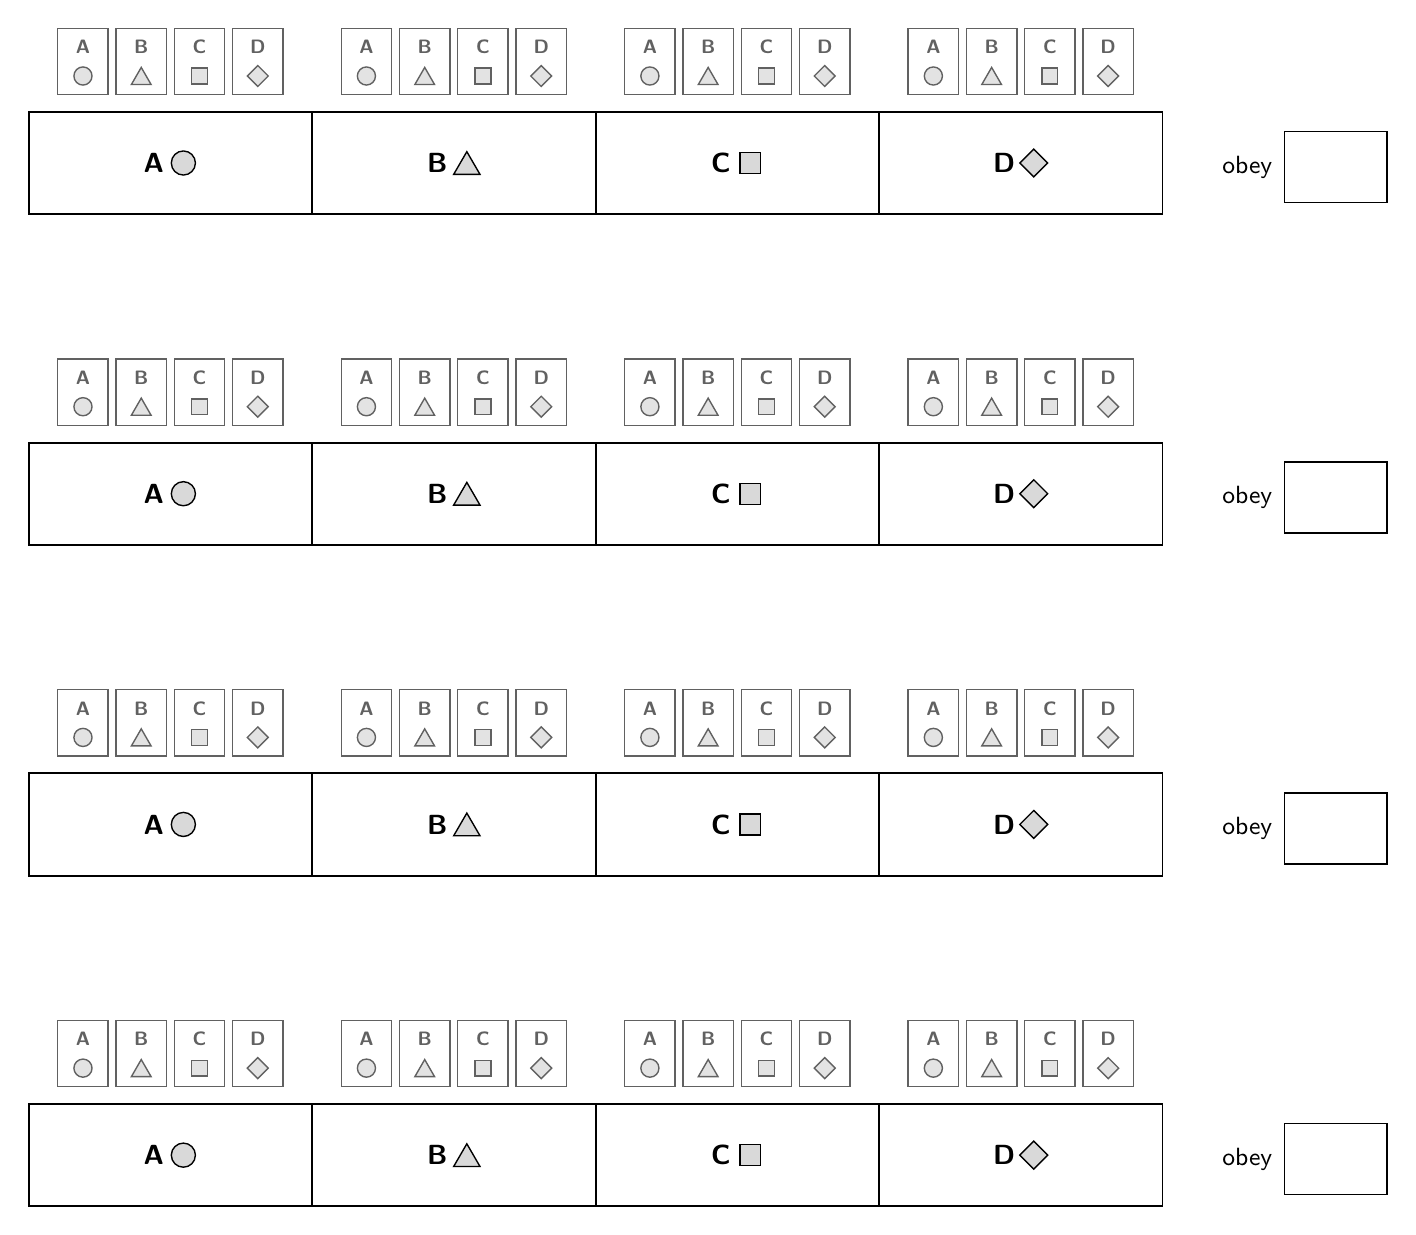
\begin{tikzpicture}[x=1mm, y=1mm]
\draw[line width=0.7pt] (0,0) rectangle (36,13);
\node[inner sep=0, font=\fontsize{10}{12.0}\selectfont\bfseries] at (15.9,6.5) {A};
\path[fill=gray!30, draw=black, line width=0.5pt] (19.65,6.5) circle (1.53);
\draw[line width=0.5pt, draw=black!62, fill=white] (3.7,15.2) rectangle (10.1,23.6);
\node[inner sep=0.5pt, fill=white, text=black!62, font=\fontsize{7}{8.4}\selectfont\bfseries] at (6.9,21.25) {A};
\path[fill=gray!22, draw=black!62, line width=0.5pt] (6.9,17.55) circle (1.15);
\draw[line width=0.5pt, draw=black!62, fill=white] (11.1,15.2) rectangle (17.5,23.6);
\node[inner sep=0.5pt, fill=white, text=black!62, font=\fontsize{7}{8.4}\selectfont\bfseries] at (14.3,21.25) {B};
\path[fill=gray!22, draw=black!62, line width=0.5pt] (14.3,18.64) -- (13.05,16.47) -- (15.55,16.47) -- cycle;
\draw[line width=0.5pt, draw=black!62, fill=white] (18.5,15.2) rectangle (24.9,23.6);
\node[inner sep=0.5pt, fill=white, text=black!62, font=\fontsize{7}{8.4}\selectfont\bfseries] at (21.7,21.25) {C};
\path[fill=gray!22, draw=black!62, line width=0.5pt] (20.7,16.55) rectangle (22.7,18.55);
\draw[line width=0.5pt, draw=black!62, fill=white] (25.9,15.2) rectangle (32.3,23.6);
\node[inner sep=0.5pt, fill=white, text=black!62, font=\fontsize{7}{8.4}\selectfont\bfseries] at (29.1,21.25) {D};
\path[fill=gray!22, draw=black!62, line width=0.5pt] (29.1,18.88) -- (30.43,17.55) -- (29.1,16.22) -- (27.77,17.55) -- cycle;
\draw[line width=0.7pt] (36,0) rectangle (72,13);
\node[inner sep=0, font=\fontsize{10}{12.0}\selectfont\bfseries] at (51.9,6.5) {B};
\path[fill=gray!30, draw=black, line width=0.5pt] (55.65,7.94) -- (53.98,5.06) -- (57.32,5.06) -- cycle;
\draw[line width=0.5pt, draw=black!62, fill=white] (39.7,15.2) rectangle (46.1,23.6);
\node[inner sep=0.5pt, fill=white, text=black!62, font=\fontsize{7}{8.4}\selectfont\bfseries] at (42.9,21.25) {A};
\path[fill=gray!22, draw=black!62, line width=0.5pt] (42.9,17.55) circle (1.15);
\draw[line width=0.5pt, draw=black!62, fill=white] (47.1,15.2) rectangle (53.5,23.6);
\node[inner sep=0.5pt, fill=white, text=black!62, font=\fontsize{7}{8.4}\selectfont\bfseries] at (50.3,21.25) {B};
\path[fill=gray!22, draw=black!62, line width=0.5pt] (50.3,18.64) -- (49.05,16.47) -- (51.55,16.47) -- cycle;
\draw[line width=0.5pt, draw=black!62, fill=white] (54.5,15.2) rectangle (60.9,23.6);
\node[inner sep=0.5pt, fill=white, text=black!62, font=\fontsize{7}{8.4}\selectfont\bfseries] at (57.7,21.25) {C};
\path[fill=gray!22, draw=black!62, line width=0.5pt] (56.7,16.55) rectangle (58.7,18.55);
\draw[line width=0.5pt, draw=black!62, fill=white] (61.9,15.2) rectangle (68.3,23.6);
\node[inner sep=0.5pt, fill=white, text=black!62, font=\fontsize{7}{8.4}\selectfont\bfseries] at (65.1,21.25) {D};
\path[fill=gray!22, draw=black!62, line width=0.5pt] (65.1,18.88) -- (66.43,17.55) -- (65.1,16.22) -- (63.77,17.55) -- cycle;
\draw[line width=0.7pt] (72,0) rectangle (108,13);
\node[inner sep=0, font=\fontsize{10}{12.0}\selectfont\bfseries] at (87.9,6.5) {C};
\path[fill=gray!30, draw=black, line width=0.5pt] (90.32,5.17) rectangle (92.98,7.83);
\draw[line width=0.5pt, draw=black!62, fill=white] (75.7,15.2) rectangle (82.1,23.6);
\node[inner sep=0.5pt, fill=white, text=black!62, font=\fontsize{7}{8.4}\selectfont\bfseries] at (78.9,21.25) {A};
\path[fill=gray!22, draw=black!62, line width=0.5pt] (78.9,17.55) circle (1.15);
\draw[line width=0.5pt, draw=black!62, fill=white] (83.1,15.2) rectangle (89.5,23.6);
\node[inner sep=0.5pt, fill=white, text=black!62, font=\fontsize{7}{8.4}\selectfont\bfseries] at (86.3,21.25) {B};
\path[fill=gray!22, draw=black!62, line width=0.5pt] (86.3,18.64) -- (85.05,16.47) -- (87.55,16.47) -- cycle;
\draw[line width=0.5pt, draw=black!62, fill=white] (90.5,15.2) rectangle (96.9,23.6);
\node[inner sep=0.5pt, fill=white, text=black!62, font=\fontsize{7}{8.4}\selectfont\bfseries] at (93.7,21.25) {C};
\path[fill=gray!22, draw=black!62, line width=0.5pt] (92.7,16.55) rectangle (94.7,18.55);
\draw[line width=0.5pt, draw=black!62, fill=white] (97.9,15.2) rectangle (104.3,23.6);
\node[inner sep=0.5pt, fill=white, text=black!62, font=\fontsize{7}{8.4}\selectfont\bfseries] at (101.1,21.25) {D};
\path[fill=gray!22, draw=black!62, line width=0.5pt] (101.1,18.88) -- (102.43,17.55) -- (101.1,16.22) -- (99.77,17.55) -- cycle;
\draw[line width=0.7pt] (108,0) rectangle (144,13);
\node[inner sep=0, font=\fontsize{10}{12.0}\selectfont\bfseries] at (123.9,6.5) {D};
\path[fill=gray!30, draw=black, line width=0.5pt] (127.65,8.27) -- (129.42,6.5) -- (127.65,4.73) -- (125.88,6.5) -- cycle;
\draw[line width=0.5pt, draw=black!62, fill=white] (111.7,15.2) rectangle (118.1,23.6);
\node[inner sep=0.5pt, fill=white, text=black!62, font=\fontsize{7}{8.4}\selectfont\bfseries] at (114.9,21.25) {A};
\path[fill=gray!22, draw=black!62, line width=0.5pt] (114.9,17.55) circle (1.15);
\draw[line width=0.5pt, draw=black!62, fill=white] (119.1,15.2) rectangle (125.5,23.6);
\node[inner sep=0.5pt, fill=white, text=black!62, font=\fontsize{7}{8.4}\selectfont\bfseries] at (122.3,21.25) {B};
\path[fill=gray!22, draw=black!62, line width=0.5pt] (122.3,18.64) -- (121.05,16.47) -- (123.55,16.47) -- cycle;
\draw[line width=0.5pt, draw=black!62, fill=white] (126.5,15.2) rectangle (132.9,23.6);
\node[inner sep=0.5pt, fill=white, text=black!62, font=\fontsize{7}{8.4}\selectfont\bfseries] at (129.7,21.25) {C};
\path[fill=gray!22, draw=black!62, line width=0.5pt] (128.7,16.55) rectangle (130.7,18.55);
\draw[line width=0.5pt, draw=black!62, fill=white] (133.9,15.2) rectangle (140.3,23.6);
\node[inner sep=0.5pt, fill=white, text=black!62, font=\fontsize{7}{8.4}\selectfont\bfseries] at (137.1,21.25) {D};
\path[fill=gray!22, draw=black!62, line width=0.5pt] (137.1,18.88) -- (138.43,17.55) -- (137.1,16.22) -- (135.77,17.55) -- cycle;
\node[anchor=east, inner sep=0, font=\fontsize{9}{10.8}\selectfont] at (158,6) {obey};
\draw[line width=0.6pt] (159.5,1.5) rectangle (172.5,10.5);
\draw[line width=0.7pt] (0,-42) rectangle (36,-29);
\node[inner sep=0, font=\fontsize{10}{12.0}\selectfont\bfseries] at (15.9,-35.5) {A};
\path[fill=gray!30, draw=black, line width=0.5pt] (19.65,-35.5) circle (1.53);
\draw[line width=0.5pt, draw=black!62, fill=white] (3.7,-26.8) rectangle (10.1,-18.4);
\node[inner sep=0.5pt, fill=white, text=black!62, font=\fontsize{7}{8.4}\selectfont\bfseries] at (6.9,-20.75) {A};
\path[fill=gray!22, draw=black!62, line width=0.5pt] (6.9,-24.45) circle (1.15);
\draw[line width=0.5pt, draw=black!62, fill=white] (11.1,-26.8) rectangle (17.5,-18.4);
\node[inner sep=0.5pt, fill=white, text=black!62, font=\fontsize{7}{8.4}\selectfont\bfseries] at (14.3,-20.75) {B};
\path[fill=gray!22, draw=black!62, line width=0.5pt] (14.3,-23.36) -- (13.05,-25.53) -- (15.55,-25.53) -- cycle;
\draw[line width=0.5pt, draw=black!62, fill=white] (18.5,-26.8) rectangle (24.9,-18.4);
\node[inner sep=0.5pt, fill=white, text=black!62, font=\fontsize{7}{8.4}\selectfont\bfseries] at (21.7,-20.75) {C};
\path[fill=gray!22, draw=black!62, line width=0.5pt] (20.7,-25.45) rectangle (22.7,-23.45);
\draw[line width=0.5pt, draw=black!62, fill=white] (25.9,-26.8) rectangle (32.3,-18.4);
\node[inner sep=0.5pt, fill=white, text=black!62, font=\fontsize{7}{8.4}\selectfont\bfseries] at (29.1,-20.75) {D};
\path[fill=gray!22, draw=black!62, line width=0.5pt] (29.1,-23.12) -- (30.43,-24.45) -- (29.1,-25.78) -- (27.77,-24.45) -- cycle;
\draw[line width=0.7pt] (36,-42) rectangle (72,-29);
\node[inner sep=0, font=\fontsize{10}{12.0}\selectfont\bfseries] at (51.9,-35.5) {B};
\path[fill=gray!30, draw=black, line width=0.5pt] (55.65,-34.06) -- (53.98,-36.94) -- (57.32,-36.94) -- cycle;
\draw[line width=0.5pt, draw=black!62, fill=white] (39.7,-26.8) rectangle (46.1,-18.4);
\node[inner sep=0.5pt, fill=white, text=black!62, font=\fontsize{7}{8.4}\selectfont\bfseries] at (42.9,-20.75) {A};
\path[fill=gray!22, draw=black!62, line width=0.5pt] (42.9,-24.45) circle (1.15);
\draw[line width=0.5pt, draw=black!62, fill=white] (47.1,-26.8) rectangle (53.5,-18.4);
\node[inner sep=0.5pt, fill=white, text=black!62, font=\fontsize{7}{8.4}\selectfont\bfseries] at (50.3,-20.75) {B};
\path[fill=gray!22, draw=black!62, line width=0.5pt] (50.3,-23.36) -- (49.05,-25.53) -- (51.55,-25.53) -- cycle;
\draw[line width=0.5pt, draw=black!62, fill=white] (54.5,-26.8) rectangle (60.9,-18.4);
\node[inner sep=0.5pt, fill=white, text=black!62, font=\fontsize{7}{8.4}\selectfont\bfseries] at (57.7,-20.75) {C};
\path[fill=gray!22, draw=black!62, line width=0.5pt] (56.7,-25.45) rectangle (58.7,-23.45);
\draw[line width=0.5pt, draw=black!62, fill=white] (61.9,-26.8) rectangle (68.3,-18.4);
\node[inner sep=0.5pt, fill=white, text=black!62, font=\fontsize{7}{8.4}\selectfont\bfseries] at (65.1,-20.75) {D};
\path[fill=gray!22, draw=black!62, line width=0.5pt] (65.1,-23.12) -- (66.43,-24.45) -- (65.1,-25.78) -- (63.77,-24.45) -- cycle;
\draw[line width=0.7pt] (72,-42) rectangle (108,-29);
\node[inner sep=0, font=\fontsize{10}{12.0}\selectfont\bfseries] at (87.9,-35.5) {C};
\path[fill=gray!30, draw=black, line width=0.5pt] (90.32,-36.83) rectangle (92.98,-34.17);
\draw[line width=0.5pt, draw=black!62, fill=white] (75.7,-26.8) rectangle (82.1,-18.4);
\node[inner sep=0.5pt, fill=white, text=black!62, font=\fontsize{7}{8.4}\selectfont\bfseries] at (78.9,-20.75) {A};
\path[fill=gray!22, draw=black!62, line width=0.5pt] (78.9,-24.45) circle (1.15);
\draw[line width=0.5pt, draw=black!62, fill=white] (83.1,-26.8) rectangle (89.5,-18.4);
\node[inner sep=0.5pt, fill=white, text=black!62, font=\fontsize{7}{8.4}\selectfont\bfseries] at (86.3,-20.75) {B};
\path[fill=gray!22, draw=black!62, line width=0.5pt] (86.3,-23.36) -- (85.05,-25.53) -- (87.55,-25.53) -- cycle;
\draw[line width=0.5pt, draw=black!62, fill=white] (90.5,-26.8) rectangle (96.9,-18.4);
\node[inner sep=0.5pt, fill=white, text=black!62, font=\fontsize{7}{8.4}\selectfont\bfseries] at (93.7,-20.75) {C};
\path[fill=gray!22, draw=black!62, line width=0.5pt] (92.7,-25.45) rectangle (94.7,-23.45);
\draw[line width=0.5pt, draw=black!62, fill=white] (97.9,-26.8) rectangle (104.3,-18.4);
\node[inner sep=0.5pt, fill=white, text=black!62, font=\fontsize{7}{8.4}\selectfont\bfseries] at (101.1,-20.75) {D};
\path[fill=gray!22, draw=black!62, line width=0.5pt] (101.1,-23.12) -- (102.43,-24.45) -- (101.1,-25.78) -- (99.77,-24.45) -- cycle;
\draw[line width=0.7pt] (108,-42) rectangle (144,-29);
\node[inner sep=0, font=\fontsize{10}{12.0}\selectfont\bfseries] at (123.9,-35.5) {D};
\path[fill=gray!30, draw=black, line width=0.5pt] (127.65,-33.73) -- (129.42,-35.5) -- (127.65,-37.27) -- (125.88,-35.5) -- cycle;
\draw[line width=0.5pt, draw=black!62, fill=white] (111.7,-26.8) rectangle (118.1,-18.4);
\node[inner sep=0.5pt, fill=white, text=black!62, font=\fontsize{7}{8.4}\selectfont\bfseries] at (114.9,-20.75) {A};
\path[fill=gray!22, draw=black!62, line width=0.5pt] (114.9,-24.45) circle (1.15);
\draw[line width=0.5pt, draw=black!62, fill=white] (119.1,-26.8) rectangle (125.5,-18.4);
\node[inner sep=0.5pt, fill=white, text=black!62, font=\fontsize{7}{8.4}\selectfont\bfseries] at (122.3,-20.75) {B};
\path[fill=gray!22, draw=black!62, line width=0.5pt] (122.3,-23.36) -- (121.05,-25.53) -- (123.55,-25.53) -- cycle;
\draw[line width=0.5pt, draw=black!62, fill=white] (126.5,-26.8) rectangle (132.9,-18.4);
\node[inner sep=0.5pt, fill=white, text=black!62, font=\fontsize{7}{8.4}\selectfont\bfseries] at (129.7,-20.75) {C};
\path[fill=gray!22, draw=black!62, line width=0.5pt] (128.7,-25.45) rectangle (130.7,-23.45);
\draw[line width=0.5pt, draw=black!62, fill=white] (133.9,-26.8) rectangle (140.3,-18.4);
\node[inner sep=0.5pt, fill=white, text=black!62, font=\fontsize{7}{8.4}\selectfont\bfseries] at (137.1,-20.75) {D};
\path[fill=gray!22, draw=black!62, line width=0.5pt] (137.1,-23.12) -- (138.43,-24.45) -- (137.1,-25.78) -- (135.77,-24.45) -- cycle;
\node[anchor=east, inner sep=0, font=\fontsize{9}{10.8}\selectfont] at (158,-36) {obey};
\draw[line width=0.6pt] (159.5,-40.5) rectangle (172.5,-31.5);
\draw[line width=0.7pt] (0,-84) rectangle (36,-71);
\node[inner sep=0, font=\fontsize{10}{12.0}\selectfont\bfseries] at (15.9,-77.5) {A};
\path[fill=gray!30, draw=black, line width=0.5pt] (19.65,-77.5) circle (1.53);
\draw[line width=0.5pt, draw=black!62, fill=white] (3.7,-68.8) rectangle (10.1,-60.4);
\node[inner sep=0.5pt, fill=white, text=black!62, font=\fontsize{7}{8.4}\selectfont\bfseries] at (6.9,-62.75) {A};
\path[fill=gray!22, draw=black!62, line width=0.5pt] (6.9,-66.45) circle (1.15);
\draw[line width=0.5pt, draw=black!62, fill=white] (11.1,-68.8) rectangle (17.5,-60.4);
\node[inner sep=0.5pt, fill=white, text=black!62, font=\fontsize{7}{8.4}\selectfont\bfseries] at (14.3,-62.75) {B};
\path[fill=gray!22, draw=black!62, line width=0.5pt] (14.3,-65.36) -- (13.05,-67.53) -- (15.55,-67.53) -- cycle;
\draw[line width=0.5pt, draw=black!62, fill=white] (18.5,-68.8) rectangle (24.9,-60.4);
\node[inner sep=0.5pt, fill=white, text=black!62, font=\fontsize{7}{8.4}\selectfont\bfseries] at (21.7,-62.75) {C};
\path[fill=gray!22, draw=black!62, line width=0.5pt] (20.7,-67.45) rectangle (22.7,-65.45);
\draw[line width=0.5pt, draw=black!62, fill=white] (25.9,-68.8) rectangle (32.3,-60.4);
\node[inner sep=0.5pt, fill=white, text=black!62, font=\fontsize{7}{8.4}\selectfont\bfseries] at (29.1,-62.75) {D};
\path[fill=gray!22, draw=black!62, line width=0.5pt] (29.1,-65.12) -- (30.43,-66.45) -- (29.1,-67.78) -- (27.77,-66.45) -- cycle;
\draw[line width=0.7pt] (36,-84) rectangle (72,-71);
\node[inner sep=0, font=\fontsize{10}{12.0}\selectfont\bfseries] at (51.9,-77.5) {B};
\path[fill=gray!30, draw=black, line width=0.5pt] (55.65,-76.06) -- (53.98,-78.94) -- (57.32,-78.94) -- cycle;
\draw[line width=0.5pt, draw=black!62, fill=white] (39.7,-68.8) rectangle (46.1,-60.4);
\node[inner sep=0.5pt, fill=white, text=black!62, font=\fontsize{7}{8.4}\selectfont\bfseries] at (42.9,-62.75) {A};
\path[fill=gray!22, draw=black!62, line width=0.5pt] (42.9,-66.45) circle (1.15);
\draw[line width=0.5pt, draw=black!62, fill=white] (47.1,-68.8) rectangle (53.5,-60.4);
\node[inner sep=0.5pt, fill=white, text=black!62, font=\fontsize{7}{8.4}\selectfont\bfseries] at (50.3,-62.75) {B};
\path[fill=gray!22, draw=black!62, line width=0.5pt] (50.3,-65.36) -- (49.05,-67.53) -- (51.55,-67.53) -- cycle;
\draw[line width=0.5pt, draw=black!62, fill=white] (54.5,-68.8) rectangle (60.9,-60.4);
\node[inner sep=0.5pt, fill=white, text=black!62, font=\fontsize{7}{8.4}\selectfont\bfseries] at (57.7,-62.75) {C};
\path[fill=gray!22, draw=black!62, line width=0.5pt] (56.7,-67.45) rectangle (58.7,-65.45);
\draw[line width=0.5pt, draw=black!62, fill=white] (61.9,-68.8) rectangle (68.3,-60.4);
\node[inner sep=0.5pt, fill=white, text=black!62, font=\fontsize{7}{8.4}\selectfont\bfseries] at (65.1,-62.75) {D};
\path[fill=gray!22, draw=black!62, line width=0.5pt] (65.1,-65.12) -- (66.43,-66.45) -- (65.1,-67.78) -- (63.77,-66.45) -- cycle;
\draw[line width=0.7pt] (72,-84) rectangle (108,-71);
\node[inner sep=0, font=\fontsize{10}{12.0}\selectfont\bfseries] at (87.9,-77.5) {C};
\path[fill=gray!30, draw=black, line width=0.5pt] (90.32,-78.83) rectangle (92.98,-76.17);
\draw[line width=0.5pt, draw=black!62, fill=white] (75.7,-68.8) rectangle (82.1,-60.4);
\node[inner sep=0.5pt, fill=white, text=black!62, font=\fontsize{7}{8.4}\selectfont\bfseries] at (78.9,-62.75) {A};
\path[fill=gray!22, draw=black!62, line width=0.5pt] (78.9,-66.45) circle (1.15);
\draw[line width=0.5pt, draw=black!62, fill=white] (83.1,-68.8) rectangle (89.5,-60.4);
\node[inner sep=0.5pt, fill=white, text=black!62, font=\fontsize{7}{8.4}\selectfont\bfseries] at (86.3,-62.75) {B};
\path[fill=gray!22, draw=black!62, line width=0.5pt] (86.3,-65.36) -- (85.05,-67.53) -- (87.55,-67.53) -- cycle;
\draw[line width=0.5pt, draw=black!62, fill=white] (90.5,-68.8) rectangle (96.9,-60.4);
\node[inner sep=0.5pt, fill=white, text=black!62, font=\fontsize{7}{8.4}\selectfont\bfseries] at (93.7,-62.75) {C};
\path[fill=gray!22, draw=black!62, line width=0.5pt] (92.7,-67.45) rectangle (94.7,-65.45);
\draw[line width=0.5pt, draw=black!62, fill=white] (97.9,-68.8) rectangle (104.3,-60.4);
\node[inner sep=0.5pt, fill=white, text=black!62, font=\fontsize{7}{8.4}\selectfont\bfseries] at (101.1,-62.75) {D};
\path[fill=gray!22, draw=black!62, line width=0.5pt] (101.1,-65.12) -- (102.43,-66.45) -- (101.1,-67.78) -- (99.77,-66.45) -- cycle;
\draw[line width=0.7pt] (108,-84) rectangle (144,-71);
\node[inner sep=0, font=\fontsize{10}{12.0}\selectfont\bfseries] at (123.9,-77.5) {D};
\path[fill=gray!30, draw=black, line width=0.5pt] (127.65,-75.73) -- (129.42,-77.5) -- (127.65,-79.27) -- (125.88,-77.5) -- cycle;
\draw[line width=0.5pt, draw=black!62, fill=white] (111.7,-68.8) rectangle (118.1,-60.4);
\node[inner sep=0.5pt, fill=white, text=black!62, font=\fontsize{7}{8.4}\selectfont\bfseries] at (114.9,-62.75) {A};
\path[fill=gray!22, draw=black!62, line width=0.5pt] (114.9,-66.45) circle (1.15);
\draw[line width=0.5pt, draw=black!62, fill=white] (119.1,-68.8) rectangle (125.5,-60.4);
\node[inner sep=0.5pt, fill=white, text=black!62, font=\fontsize{7}{8.4}\selectfont\bfseries] at (122.3,-62.75) {B};
\path[fill=gray!22, draw=black!62, line width=0.5pt] (122.3,-65.36) -- (121.05,-67.53) -- (123.55,-67.53) -- cycle;
\draw[line width=0.5pt, draw=black!62, fill=white] (126.5,-68.8) rectangle (132.9,-60.4);
\node[inner sep=0.5pt, fill=white, text=black!62, font=\fontsize{7}{8.4}\selectfont\bfseries] at (129.7,-62.75) {C};
\path[fill=gray!22, draw=black!62, line width=0.5pt] (128.7,-67.45) rectangle (130.7,-65.45);
\draw[line width=0.5pt, draw=black!62, fill=white] (133.9,-68.8) rectangle (140.3,-60.4);
\node[inner sep=0.5pt, fill=white, text=black!62, font=\fontsize{7}{8.4}\selectfont\bfseries] at (137.1,-62.75) {D};
\path[fill=gray!22, draw=black!62, line width=0.5pt] (137.1,-65.12) -- (138.43,-66.45) -- (137.1,-67.78) -- (135.77,-66.45) -- cycle;
\node[anchor=east, inner sep=0, font=\fontsize{9}{10.8}\selectfont] at (158,-78) {obey};
\draw[line width=0.6pt] (159.5,-82.5) rectangle (172.5,-73.5);
\draw[line width=0.7pt] (0,-126) rectangle (36,-113);
\node[inner sep=0, font=\fontsize{10}{12.0}\selectfont\bfseries] at (15.9,-119.5) {A};
\path[fill=gray!30, draw=black, line width=0.5pt] (19.65,-119.5) circle (1.53);
\draw[line width=0.5pt, draw=black!62, fill=white] (3.7,-110.8) rectangle (10.1,-102.4);
\node[inner sep=0.5pt, fill=white, text=black!62, font=\fontsize{7}{8.4}\selectfont\bfseries] at (6.9,-104.75) {A};
\path[fill=gray!22, draw=black!62, line width=0.5pt] (6.9,-108.45) circle (1.15);
\draw[line width=0.5pt, draw=black!62, fill=white] (11.1,-110.8) rectangle (17.5,-102.4);
\node[inner sep=0.5pt, fill=white, text=black!62, font=\fontsize{7}{8.4}\selectfont\bfseries] at (14.3,-104.75) {B};
\path[fill=gray!22, draw=black!62, line width=0.5pt] (14.3,-107.36) -- (13.05,-109.53) -- (15.55,-109.53) -- cycle;
\draw[line width=0.5pt, draw=black!62, fill=white] (18.5,-110.8) rectangle (24.9,-102.4);
\node[inner sep=0.5pt, fill=white, text=black!62, font=\fontsize{7}{8.4}\selectfont\bfseries] at (21.7,-104.75) {C};
\path[fill=gray!22, draw=black!62, line width=0.5pt] (20.7,-109.45) rectangle (22.7,-107.45);
\draw[line width=0.5pt, draw=black!62, fill=white] (25.9,-110.8) rectangle (32.3,-102.4);
\node[inner sep=0.5pt, fill=white, text=black!62, font=\fontsize{7}{8.4}\selectfont\bfseries] at (29.1,-104.75) {D};
\path[fill=gray!22, draw=black!62, line width=0.5pt] (29.1,-107.12) -- (30.43,-108.45) -- (29.1,-109.78) -- (27.77,-108.45) -- cycle;
\draw[line width=0.7pt] (36,-126) rectangle (72,-113);
\node[inner sep=0, font=\fontsize{10}{12.0}\selectfont\bfseries] at (51.9,-119.5) {B};
\path[fill=gray!30, draw=black, line width=0.5pt] (55.65,-118.06) -- (53.98,-120.94) -- (57.32,-120.94) -- cycle;
\draw[line width=0.5pt, draw=black!62, fill=white] (39.7,-110.8) rectangle (46.1,-102.4);
\node[inner sep=0.5pt, fill=white, text=black!62, font=\fontsize{7}{8.4}\selectfont\bfseries] at (42.9,-104.75) {A};
\path[fill=gray!22, draw=black!62, line width=0.5pt] (42.9,-108.45) circle (1.15);
\draw[line width=0.5pt, draw=black!62, fill=white] (47.1,-110.8) rectangle (53.5,-102.4);
\node[inner sep=0.5pt, fill=white, text=black!62, font=\fontsize{7}{8.4}\selectfont\bfseries] at (50.3,-104.75) {B};
\path[fill=gray!22, draw=black!62, line width=0.5pt] (50.3,-107.36) -- (49.05,-109.53) -- (51.55,-109.53) -- cycle;
\draw[line width=0.5pt, draw=black!62, fill=white] (54.5,-110.8) rectangle (60.9,-102.4);
\node[inner sep=0.5pt, fill=white, text=black!62, font=\fontsize{7}{8.4}\selectfont\bfseries] at (57.7,-104.75) {C};
\path[fill=gray!22, draw=black!62, line width=0.5pt] (56.7,-109.45) rectangle (58.7,-107.45);
\draw[line width=0.5pt, draw=black!62, fill=white] (61.9,-110.8) rectangle (68.3,-102.4);
\node[inner sep=0.5pt, fill=white, text=black!62, font=\fontsize{7}{8.4}\selectfont\bfseries] at (65.1,-104.75) {D};
\path[fill=gray!22, draw=black!62, line width=0.5pt] (65.1,-107.12) -- (66.43,-108.45) -- (65.1,-109.78) -- (63.77,-108.45) -- cycle;
\draw[line width=0.7pt] (72,-126) rectangle (108,-113);
\node[inner sep=0, font=\fontsize{10}{12.0}\selectfont\bfseries] at (87.9,-119.5) {C};
\path[fill=gray!30, draw=black, line width=0.5pt] (90.32,-120.83) rectangle (92.98,-118.17);
\draw[line width=0.5pt, draw=black!62, fill=white] (75.7,-110.8) rectangle (82.1,-102.4);
\node[inner sep=0.5pt, fill=white, text=black!62, font=\fontsize{7}{8.4}\selectfont\bfseries] at (78.9,-104.75) {A};
\path[fill=gray!22, draw=black!62, line width=0.5pt] (78.9,-108.45) circle (1.15);
\draw[line width=0.5pt, draw=black!62, fill=white] (83.1,-110.8) rectangle (89.5,-102.4);
\node[inner sep=0.5pt, fill=white, text=black!62, font=\fontsize{7}{8.4}\selectfont\bfseries] at (86.3,-104.75) {B};
\path[fill=gray!22, draw=black!62, line width=0.5pt] (86.3,-107.36) -- (85.05,-109.53) -- (87.55,-109.53) -- cycle;
\draw[line width=0.5pt, draw=black!62, fill=white] (90.5,-110.8) rectangle (96.9,-102.4);
\node[inner sep=0.5pt, fill=white, text=black!62, font=\fontsize{7}{8.4}\selectfont\bfseries] at (93.7,-104.75) {C};
\path[fill=gray!22, draw=black!62, line width=0.5pt] (92.7,-109.45) rectangle (94.7,-107.45);
\draw[line width=0.5pt, draw=black!62, fill=white] (97.9,-110.8) rectangle (104.3,-102.4);
\node[inner sep=0.5pt, fill=white, text=black!62, font=\fontsize{7}{8.4}\selectfont\bfseries] at (101.1,-104.75) {D};
\path[fill=gray!22, draw=black!62, line width=0.5pt] (101.1,-107.12) -- (102.43,-108.45) -- (101.1,-109.78) -- (99.77,-108.45) -- cycle;
\draw[line width=0.7pt] (108,-126) rectangle (144,-113);
\node[inner sep=0, font=\fontsize{10}{12.0}\selectfont\bfseries] at (123.9,-119.5) {D};
\path[fill=gray!30, draw=black, line width=0.5pt] (127.65,-117.73) -- (129.42,-119.5) -- (127.65,-121.27) -- (125.88,-119.5) -- cycle;
\draw[line width=0.5pt, draw=black!62, fill=white] (111.7,-110.8) rectangle (118.1,-102.4);
\node[inner sep=0.5pt, fill=white, text=black!62, font=\fontsize{7}{8.4}\selectfont\bfseries] at (114.9,-104.75) {A};
\path[fill=gray!22, draw=black!62, line width=0.5pt] (114.9,-108.45) circle (1.15);
\draw[line width=0.5pt, draw=black!62, fill=white] (119.1,-110.8) rectangle (125.5,-102.4);
\node[inner sep=0.5pt, fill=white, text=black!62, font=\fontsize{7}{8.4}\selectfont\bfseries] at (122.3,-104.75) {B};
\path[fill=gray!22, draw=black!62, line width=0.5pt] (122.3,-107.36) -- (121.05,-109.53) -- (123.55,-109.53) -- cycle;
\draw[line width=0.5pt, draw=black!62, fill=white] (126.5,-110.8) rectangle (132.9,-102.4);
\node[inner sep=0.5pt, fill=white, text=black!62, font=\fontsize{7}{8.4}\selectfont\bfseries] at (129.7,-104.75) {C};
\path[fill=gray!22, draw=black!62, line width=0.5pt] (128.7,-109.45) rectangle (130.7,-107.45);
\draw[line width=0.5pt, draw=black!62, fill=white] (133.9,-110.8) rectangle (140.3,-102.4);
\node[inner sep=0.5pt, fill=white, text=black!62, font=\fontsize{7}{8.4}\selectfont\bfseries] at (137.1,-104.75) {D};
\path[fill=gray!22, draw=black!62, line width=0.5pt] (137.1,-107.12) -- (138.43,-108.45) -- (137.1,-109.78) -- (135.77,-108.45) -- cycle;
\node[anchor=east, inner sep=0, font=\fontsize{9}{10.8}\selectfont] at (158,-120) {obey};
\draw[line width=0.6pt] (159.5,-124.5) rectangle (172.5,-115.5);
\end{tikzpicture}\par

\vfill

\end{document}
